(g). (4 points) \textsl{While centrality helps explain the evolution of every player's role individually, we need to explore the global trends and incidents in the story in order to understand the behavior of the criminal enterprise.}\\
\textsl{Describe the coarse pattern(s) you observe as the network evolves through the phases. Does the network evolution reflect the background story? ($\sim$200 words, 300 word limit.)}\\

\textbf{Solution}:\\
As mentioned before in part (c), the number of edges is not further increasing after phase 4, whereas the number of nodes is slowly increasing until it reaches a plateau-like boundary at phase 8 (see figure \ref{fig:nodes_edges}). This development can visually be shown in figure \ref{fig:network_visualization}. Generally there is a development that the network decentralizes over the phases and its main actor (node no. 1) looses his importance according to the betweenness centrality (see figure \ref{fig:betweenness_specific_nodes}). The seizures seem to have some impact on the structure of the graph.\\

\begin{figure}[htbp]
	\centering
	\begin{minipage}{.24\textwidth}
		\centering
		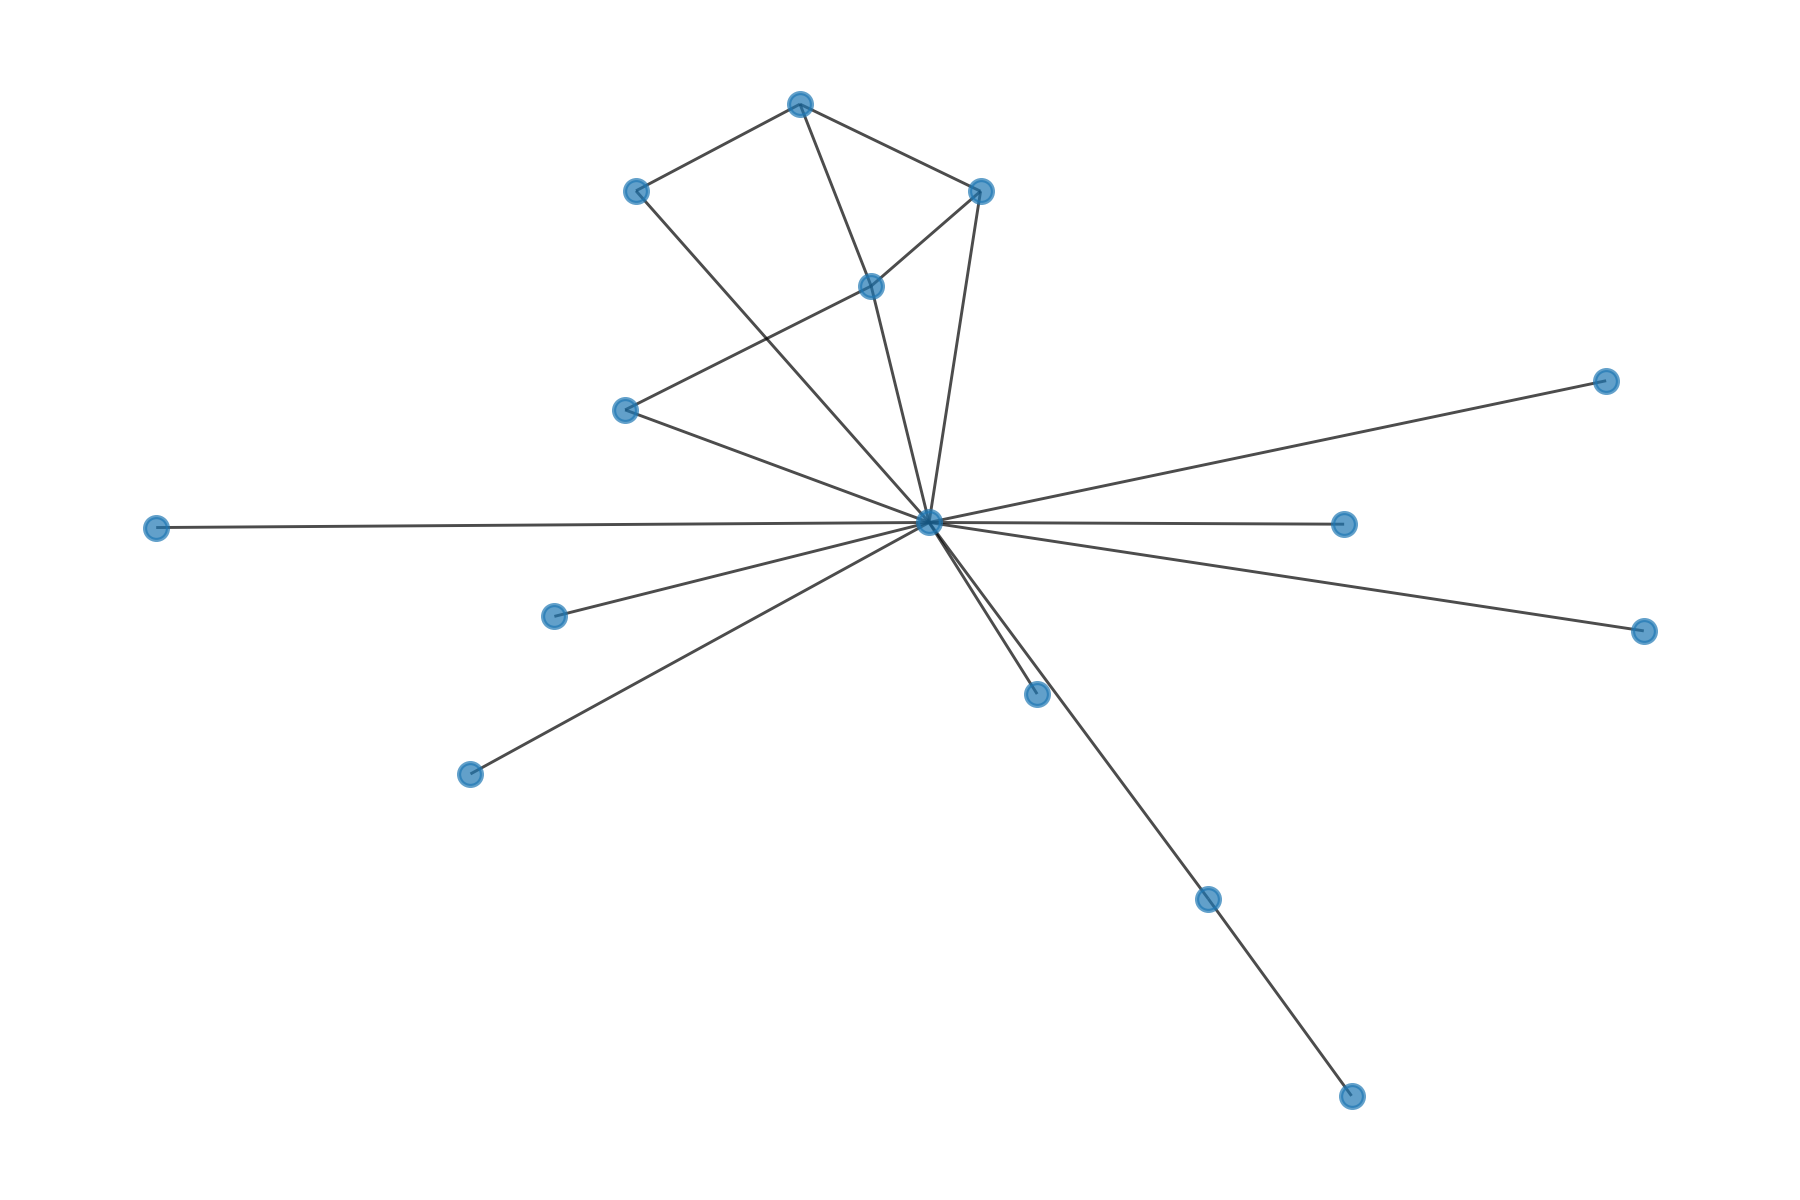
\includegraphics[width=1\linewidth]{problem_02/network_phase1}
	\end{minipage}
	\begin{minipage}{.24\textwidth}
		\centering
		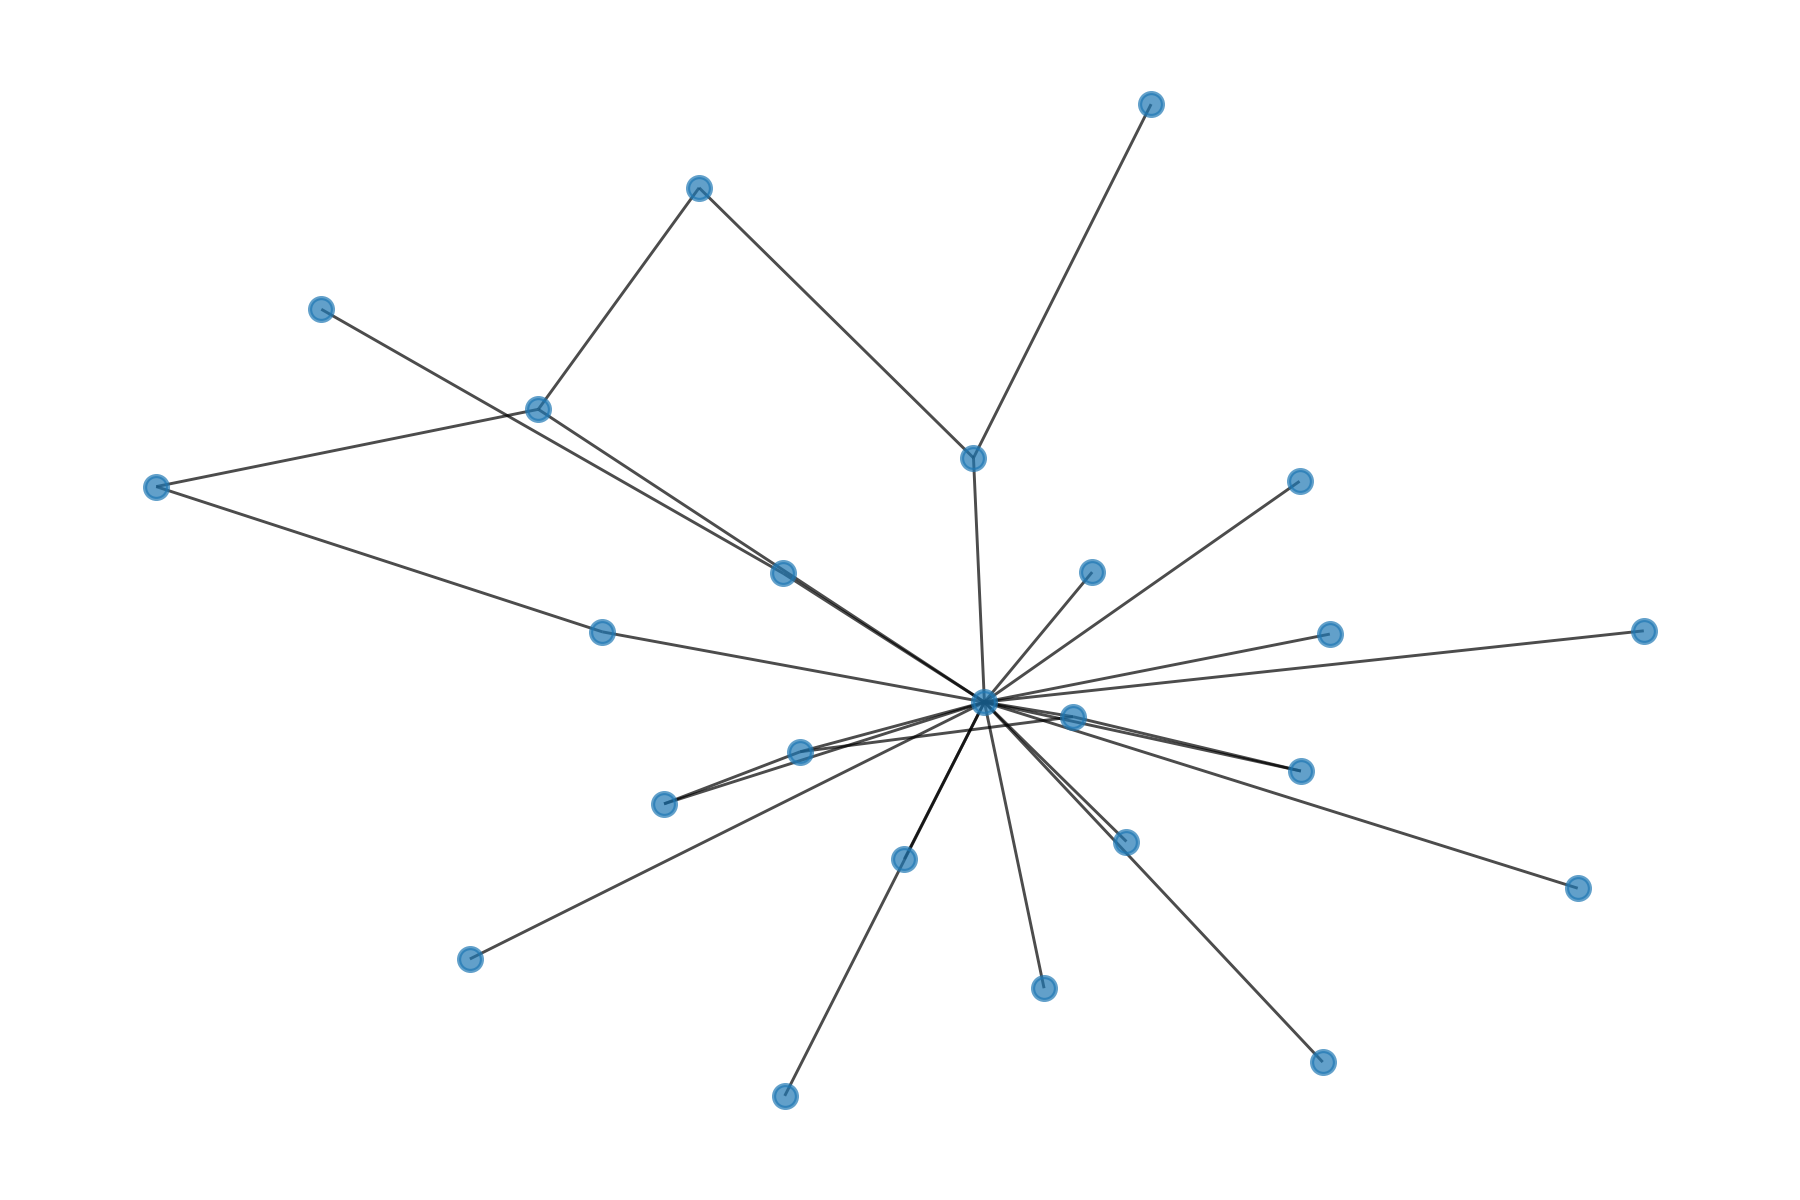
\includegraphics[width=1\linewidth]{problem_02/network_phase2}
	\end{minipage}
	\begin{minipage}{.24\textwidth}
		\centering
		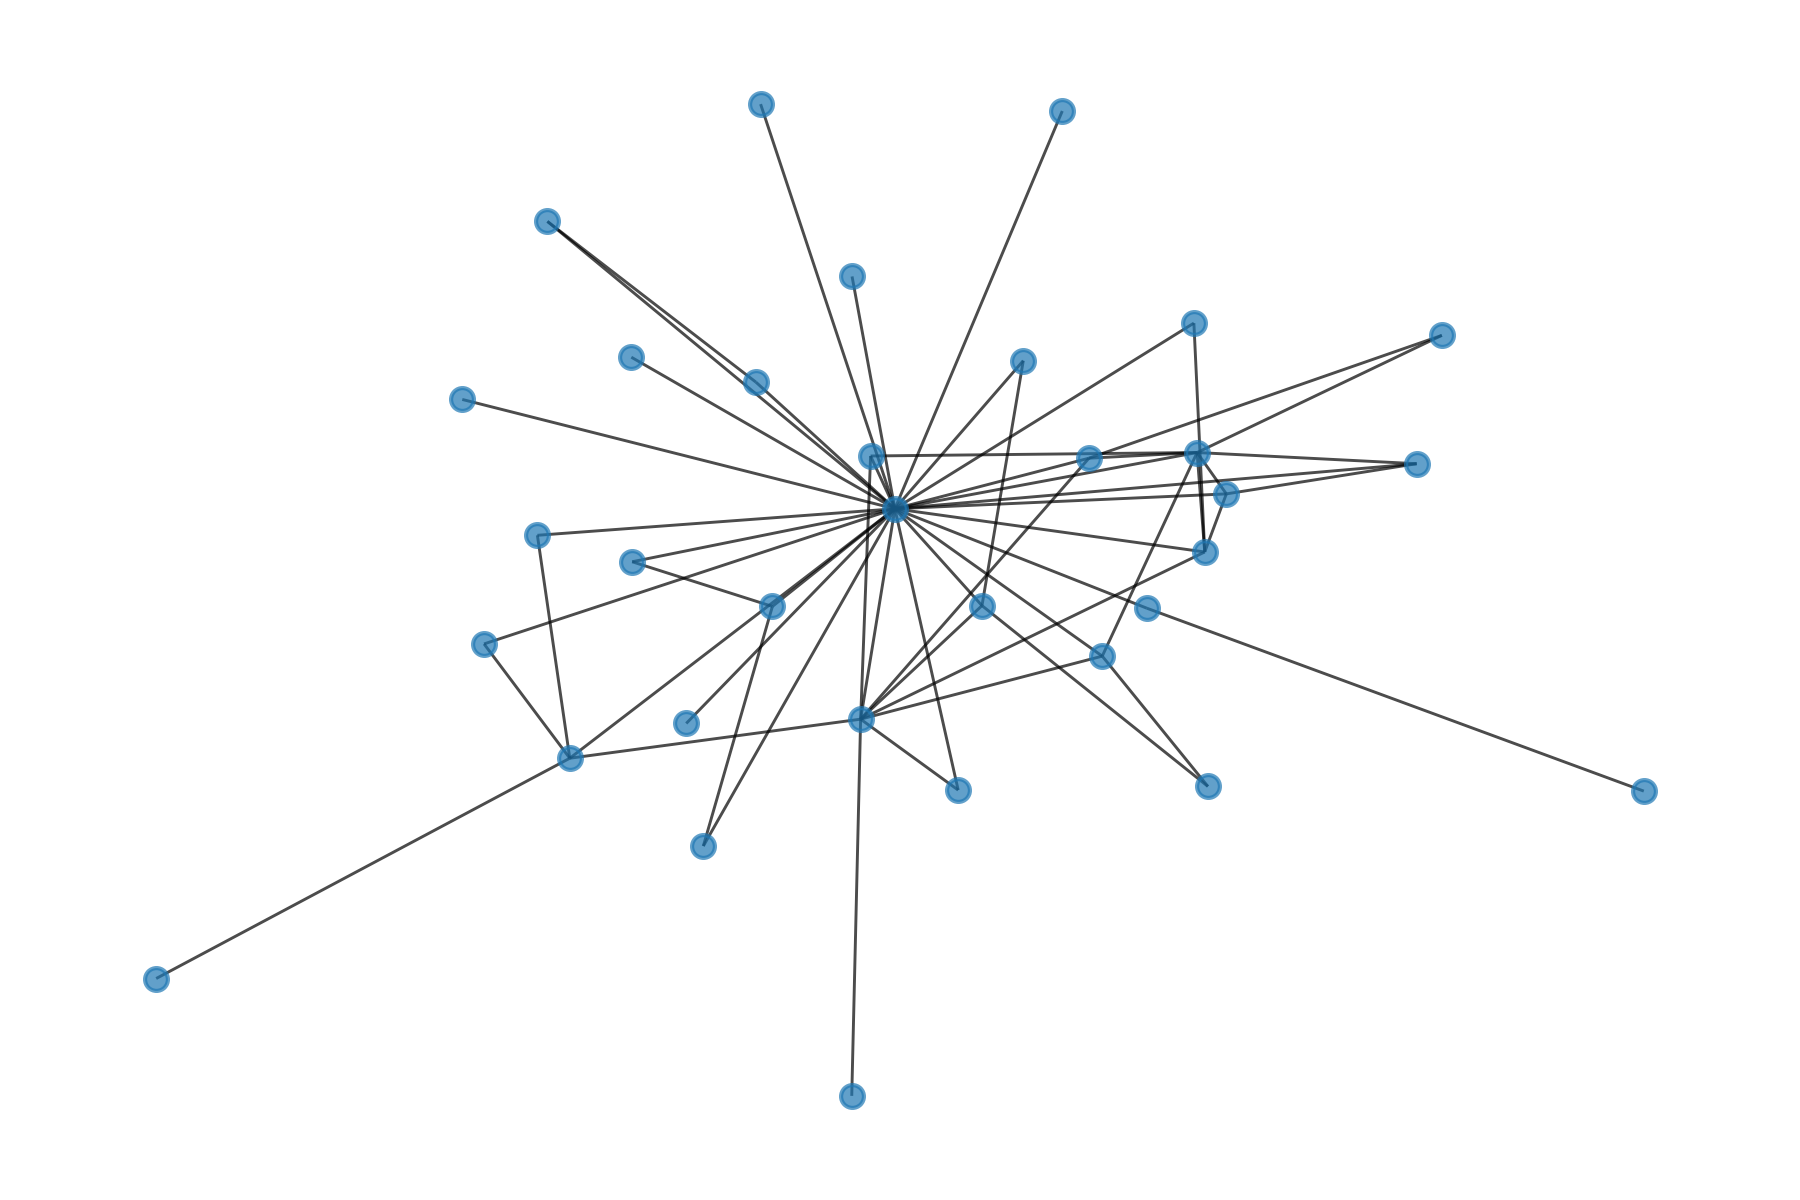
\includegraphics[width=1\linewidth]{problem_02/network_phase3}
	\end{minipage}
	\begin{minipage}{.24\textwidth}
		\centering
		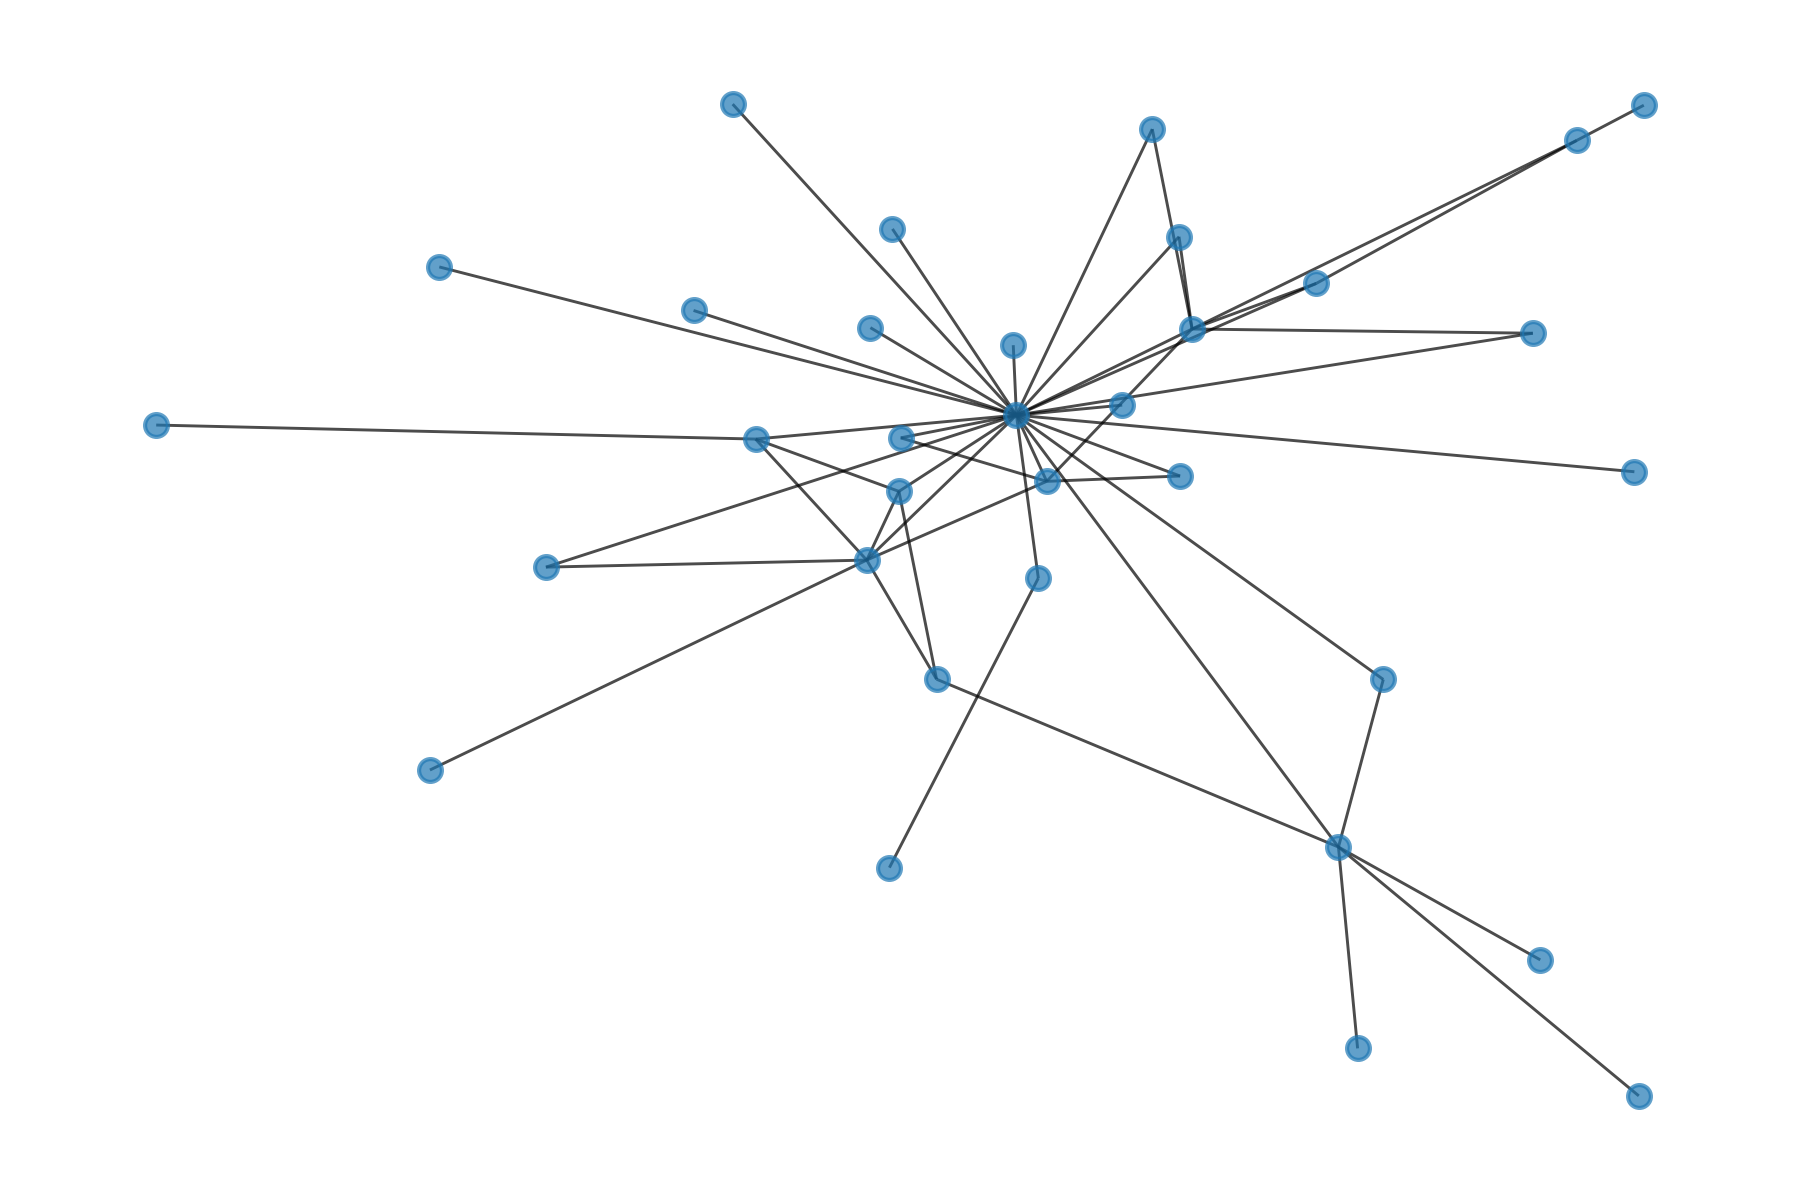
\includegraphics[width=1\linewidth]{problem_02/network_phase4}
	\end{minipage}
		\begin{minipage}{.24\textwidth}
		\centering
		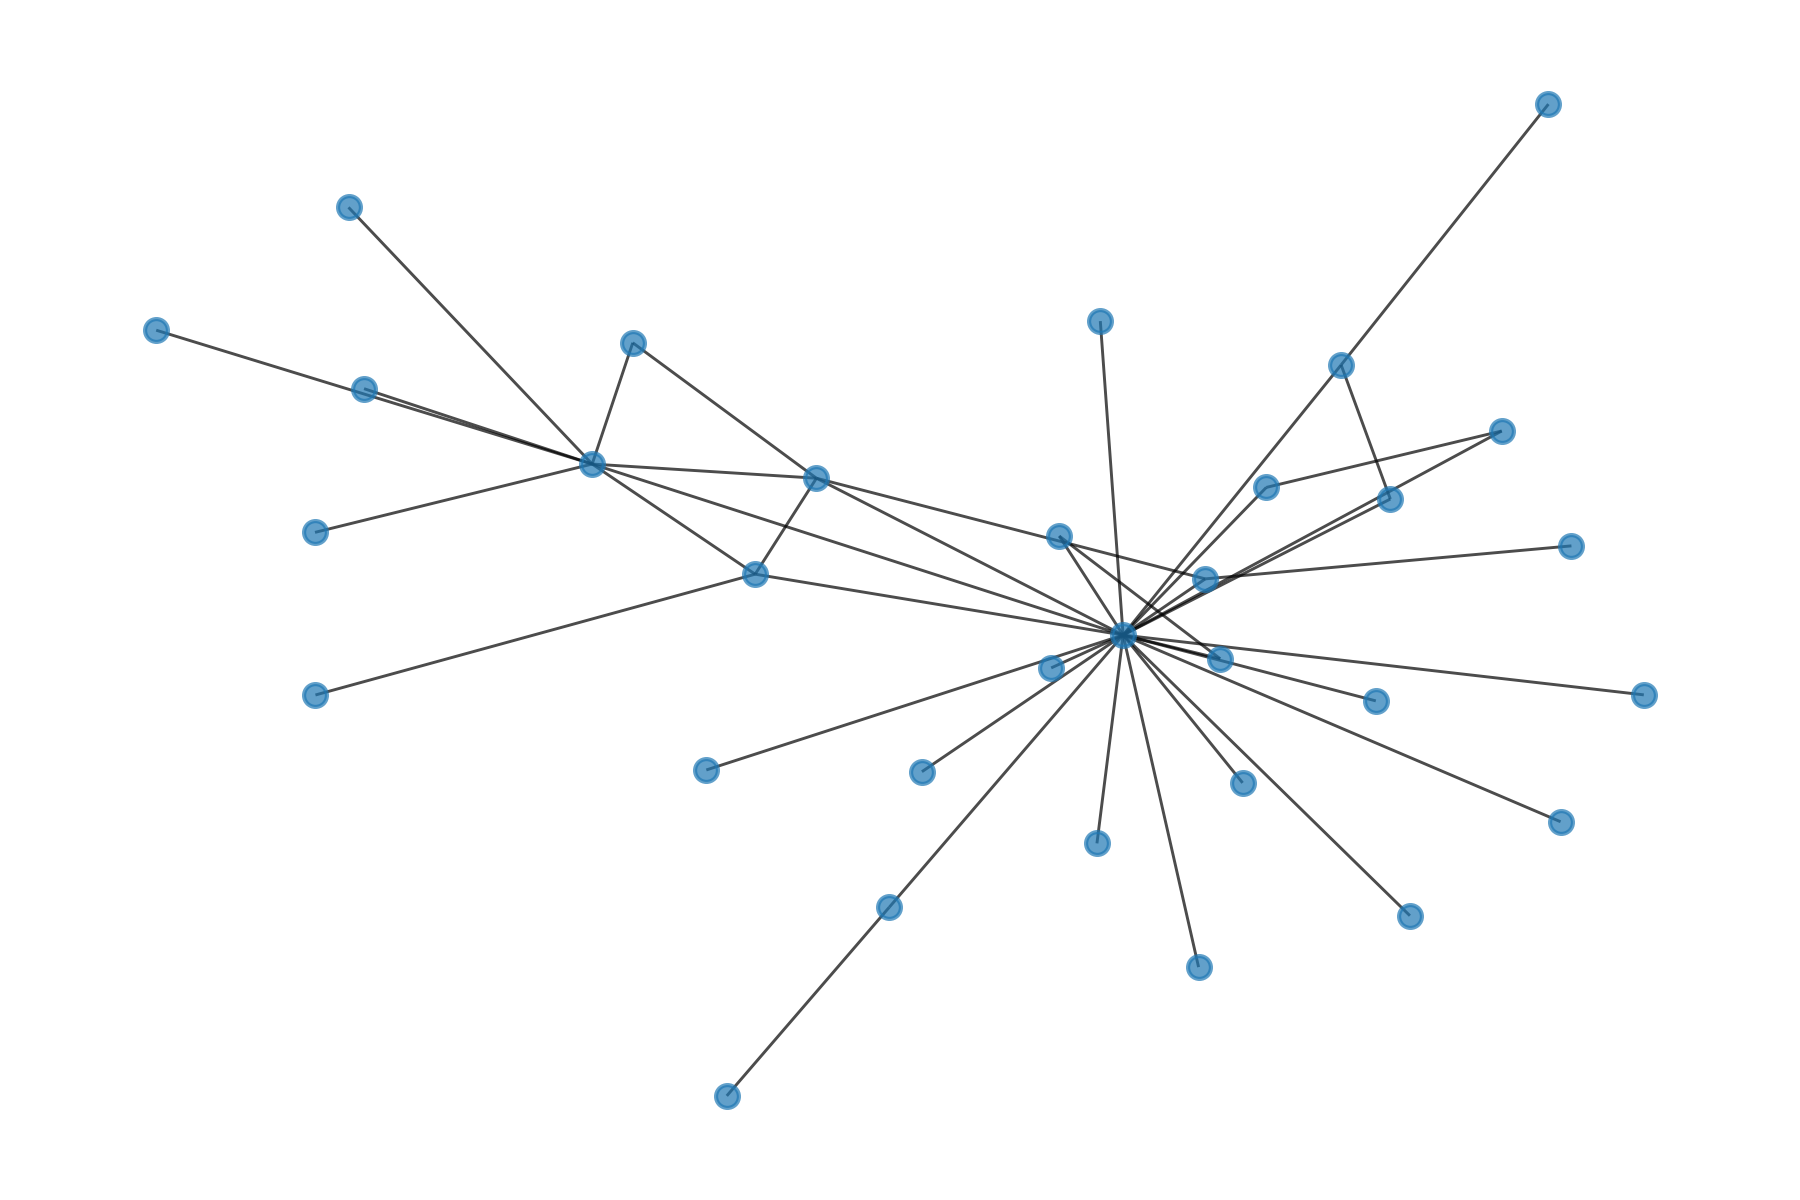
\includegraphics[width=1\linewidth]{problem_02/network_phase5}
	\end{minipage}
	\begin{minipage}{.24\textwidth}
		\centering
		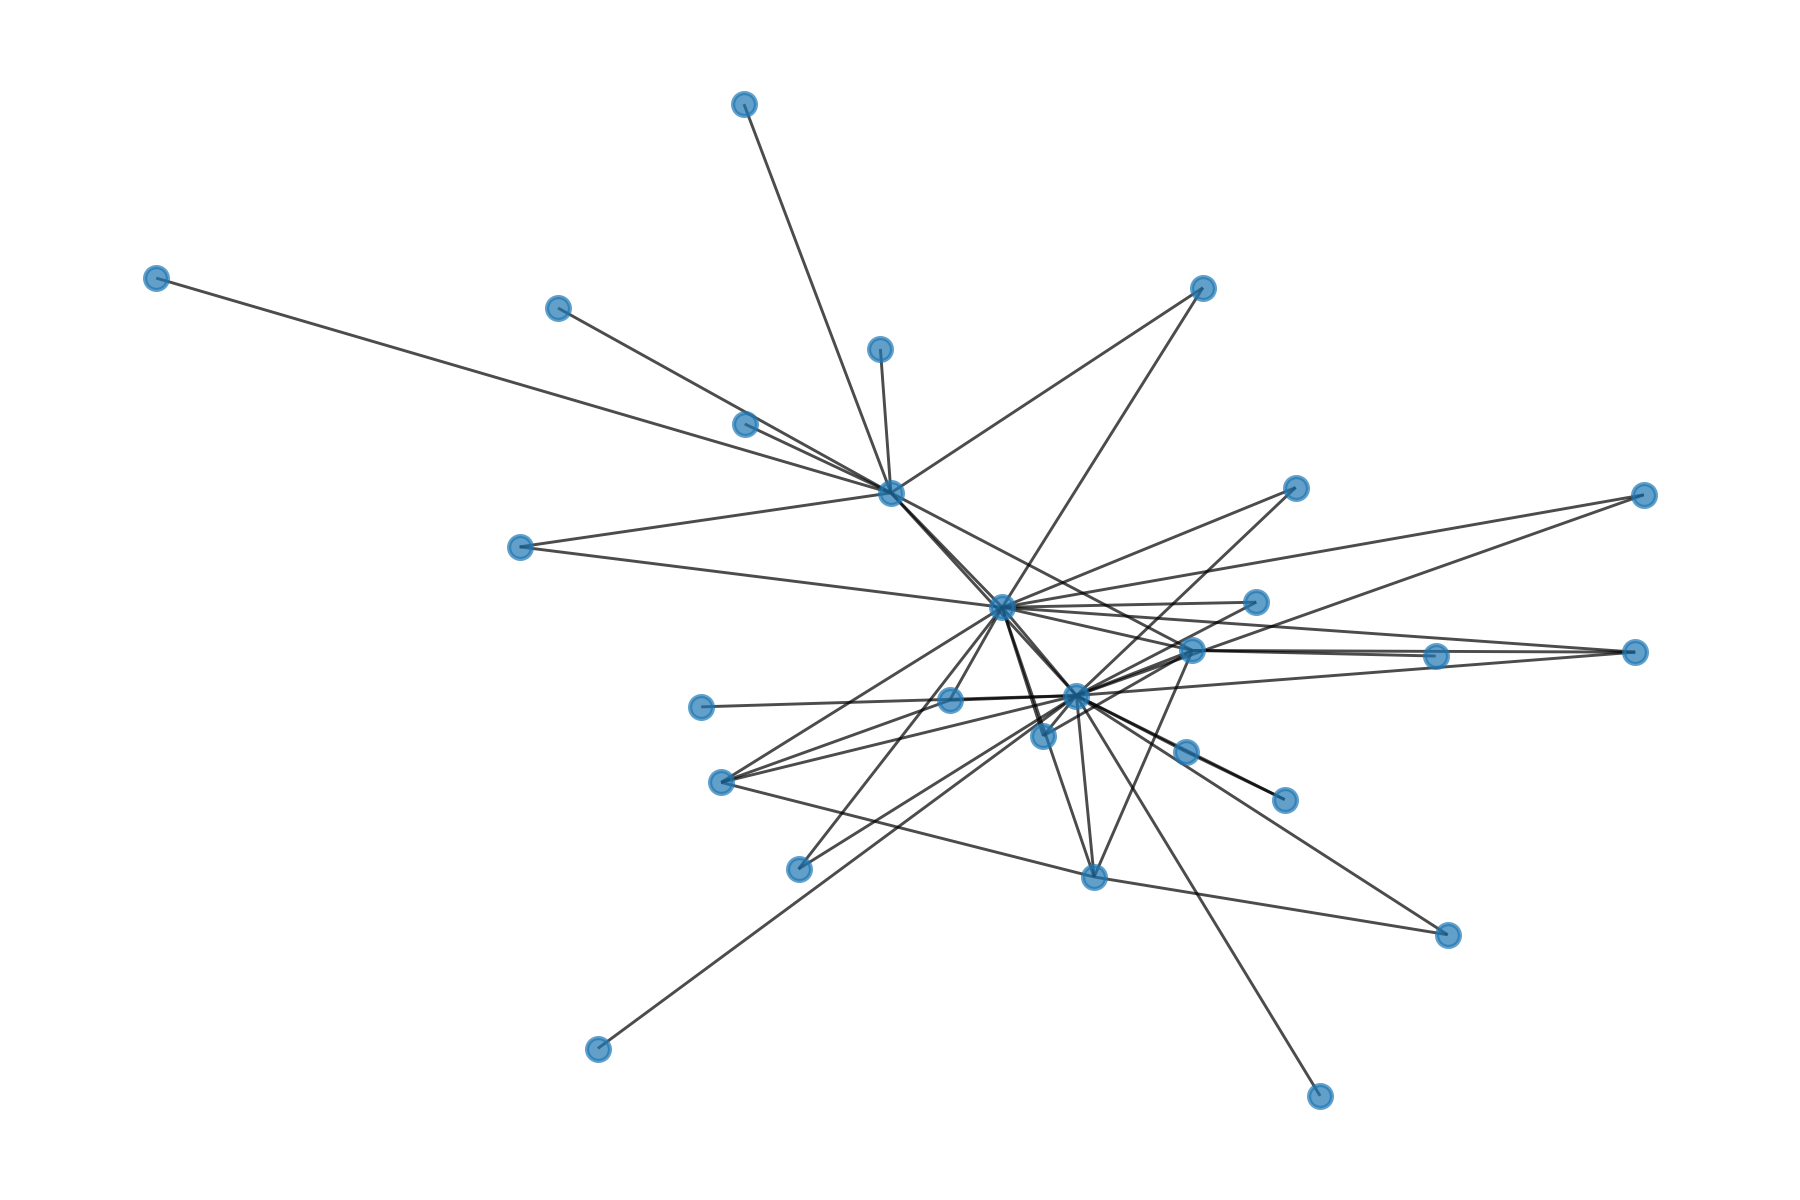
\includegraphics[width=1\linewidth]{problem_02/network_phase6}
	\end{minipage}
	\begin{minipage}{.24\textwidth}
		\centering
		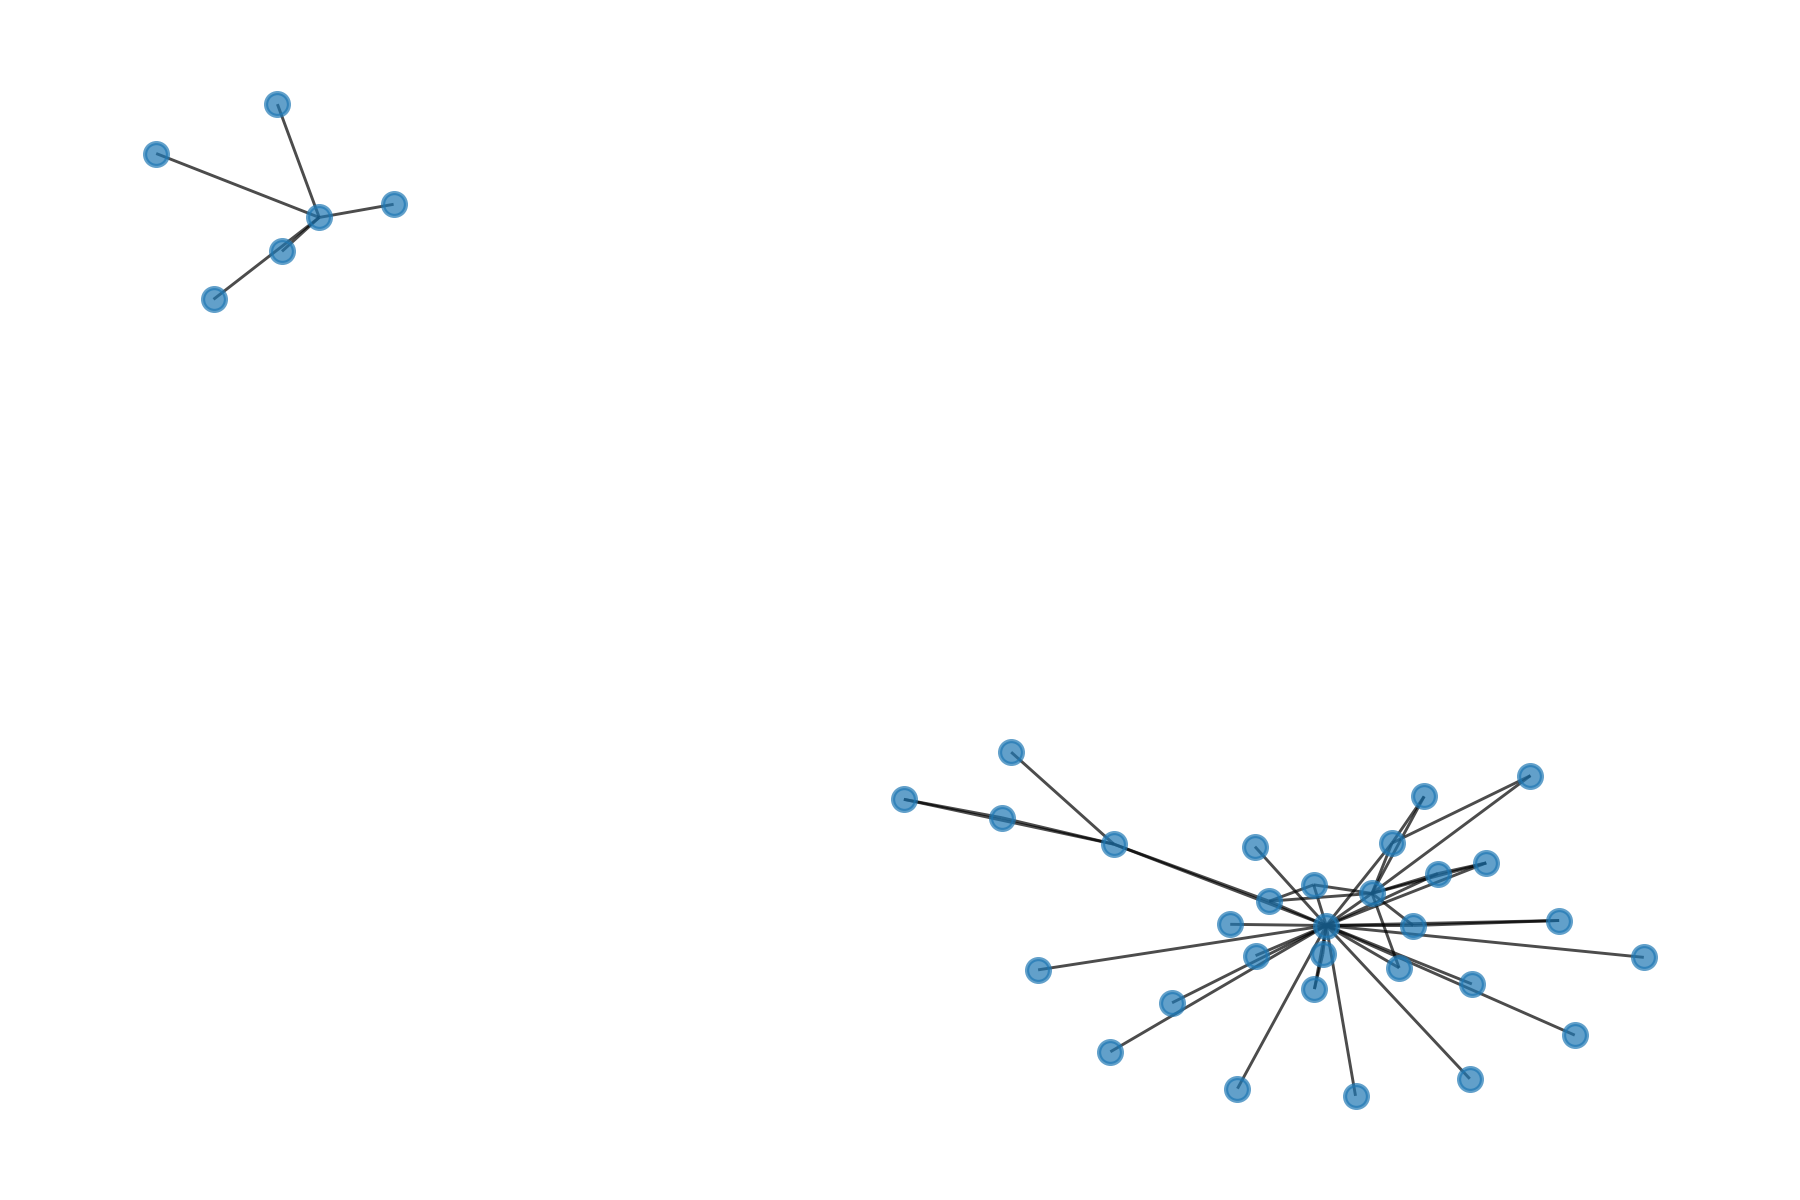
\includegraphics[width=1\linewidth]{problem_02/network_phase7}
	\end{minipage}
	\begin{minipage}{.24\textwidth}
		\centering
		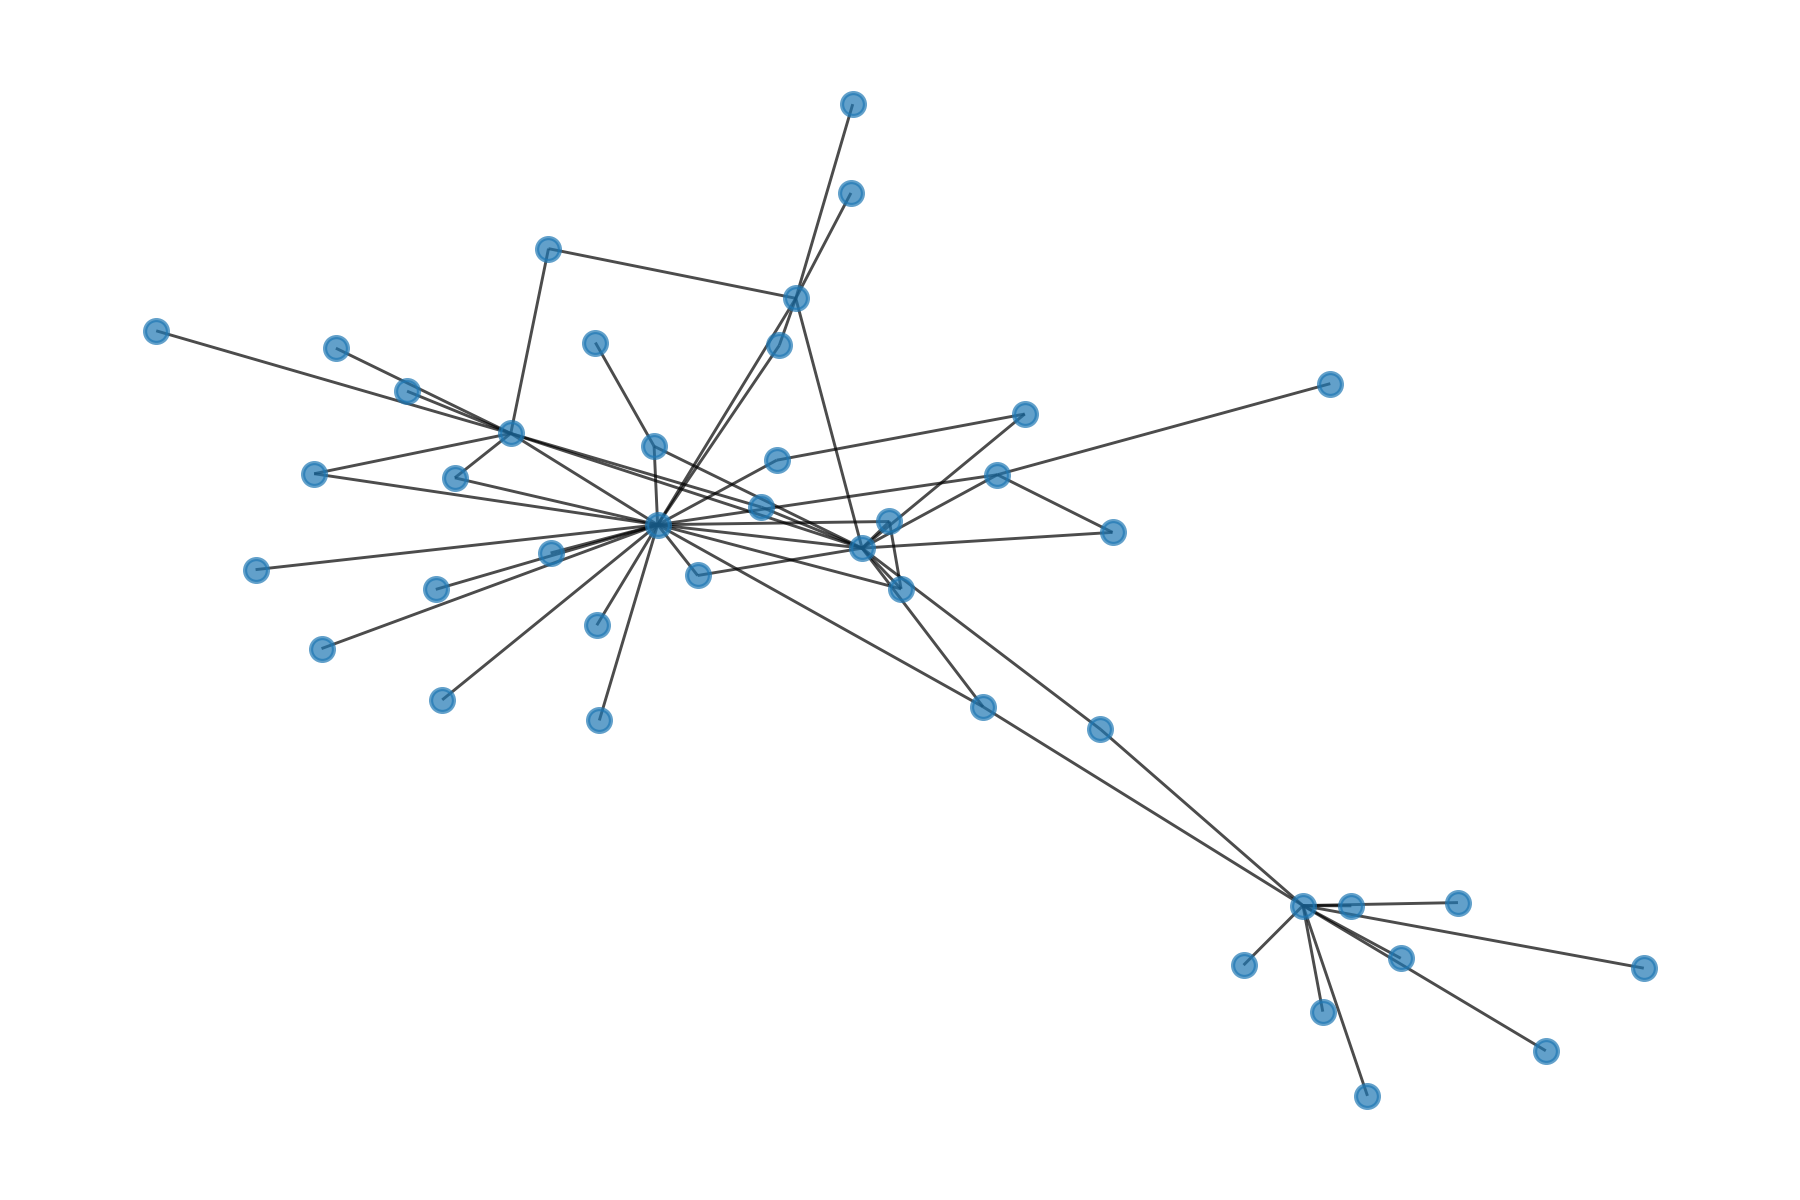
\includegraphics[width=1\linewidth]{problem_02/network_phase8}
	\end{minipage}
	\begin{minipage}{.24\textwidth}
		\centering
		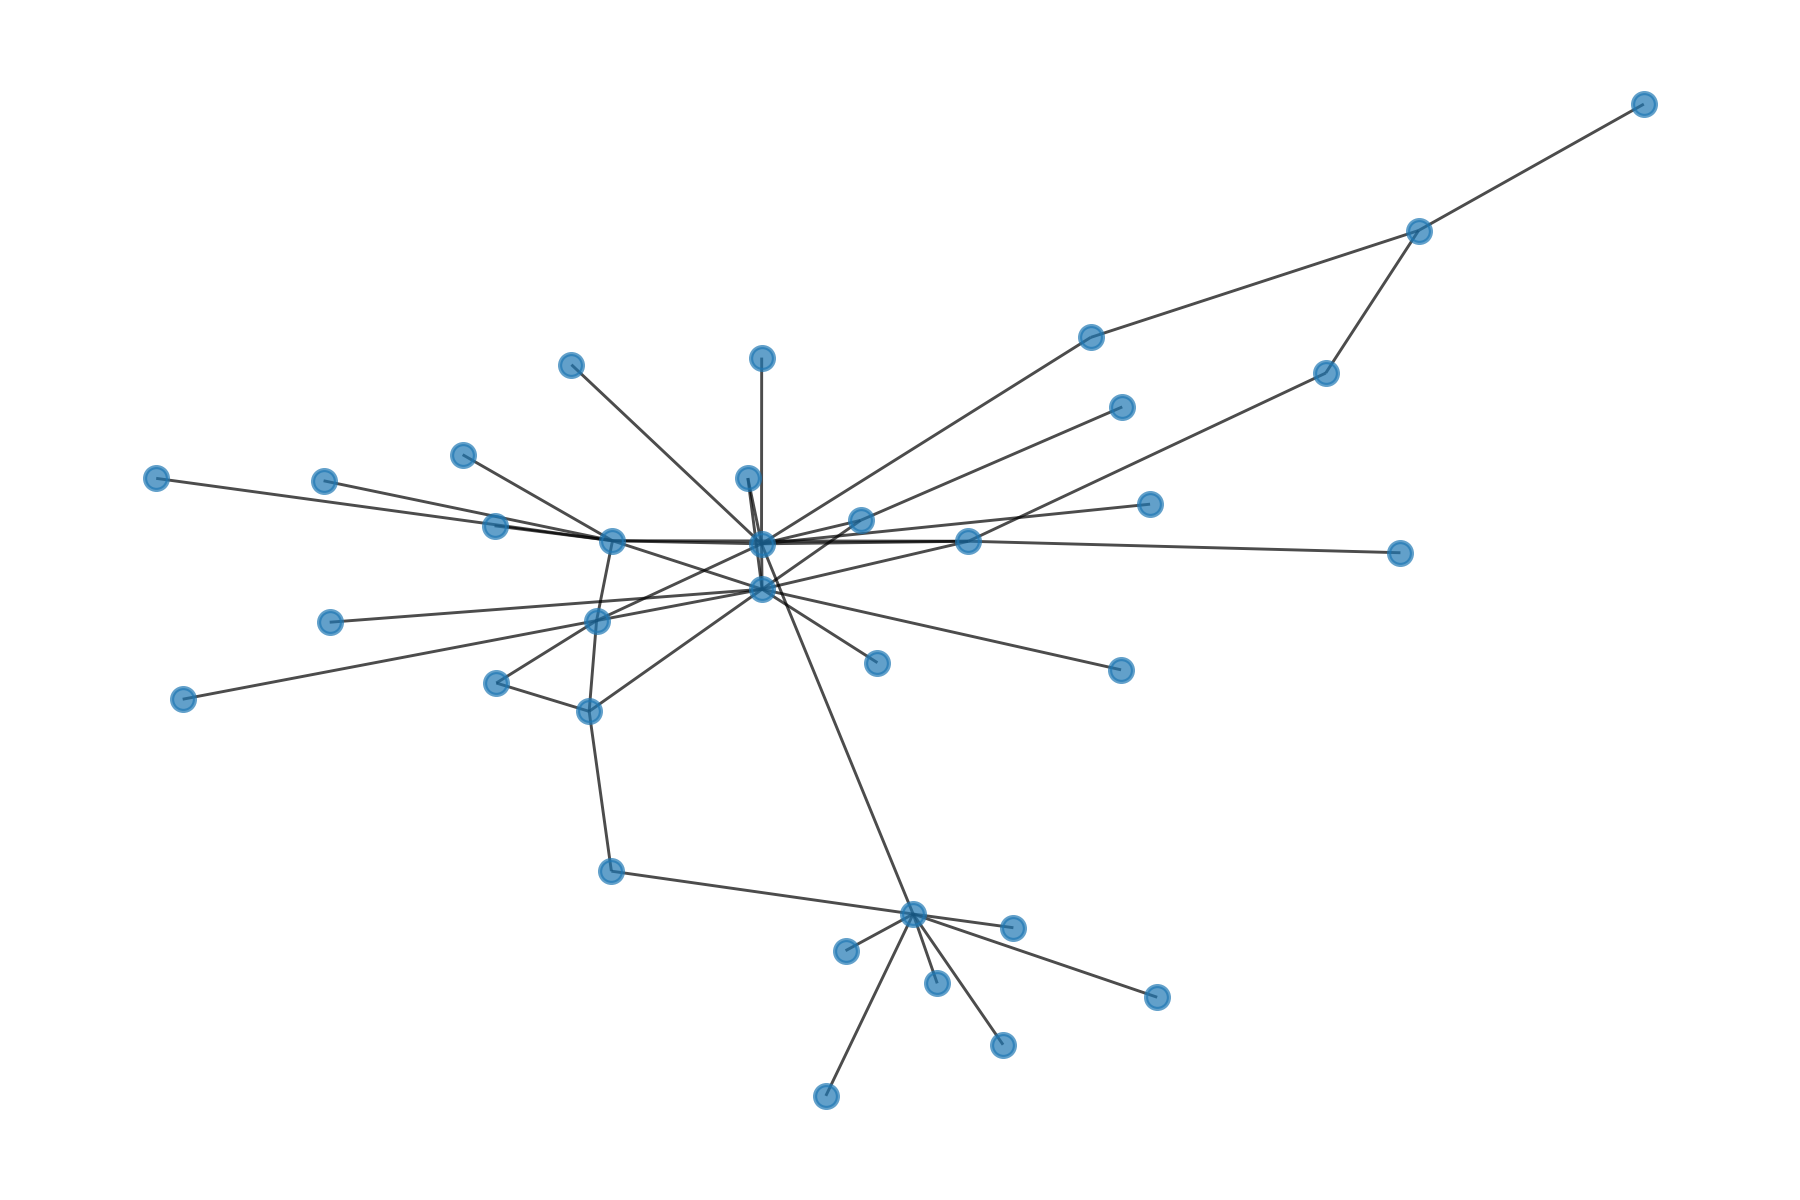
\includegraphics[width=1\linewidth]{problem_02/network_phase9}
	\end{minipage}
	\begin{minipage}{.24\textwidth}
		\centering
		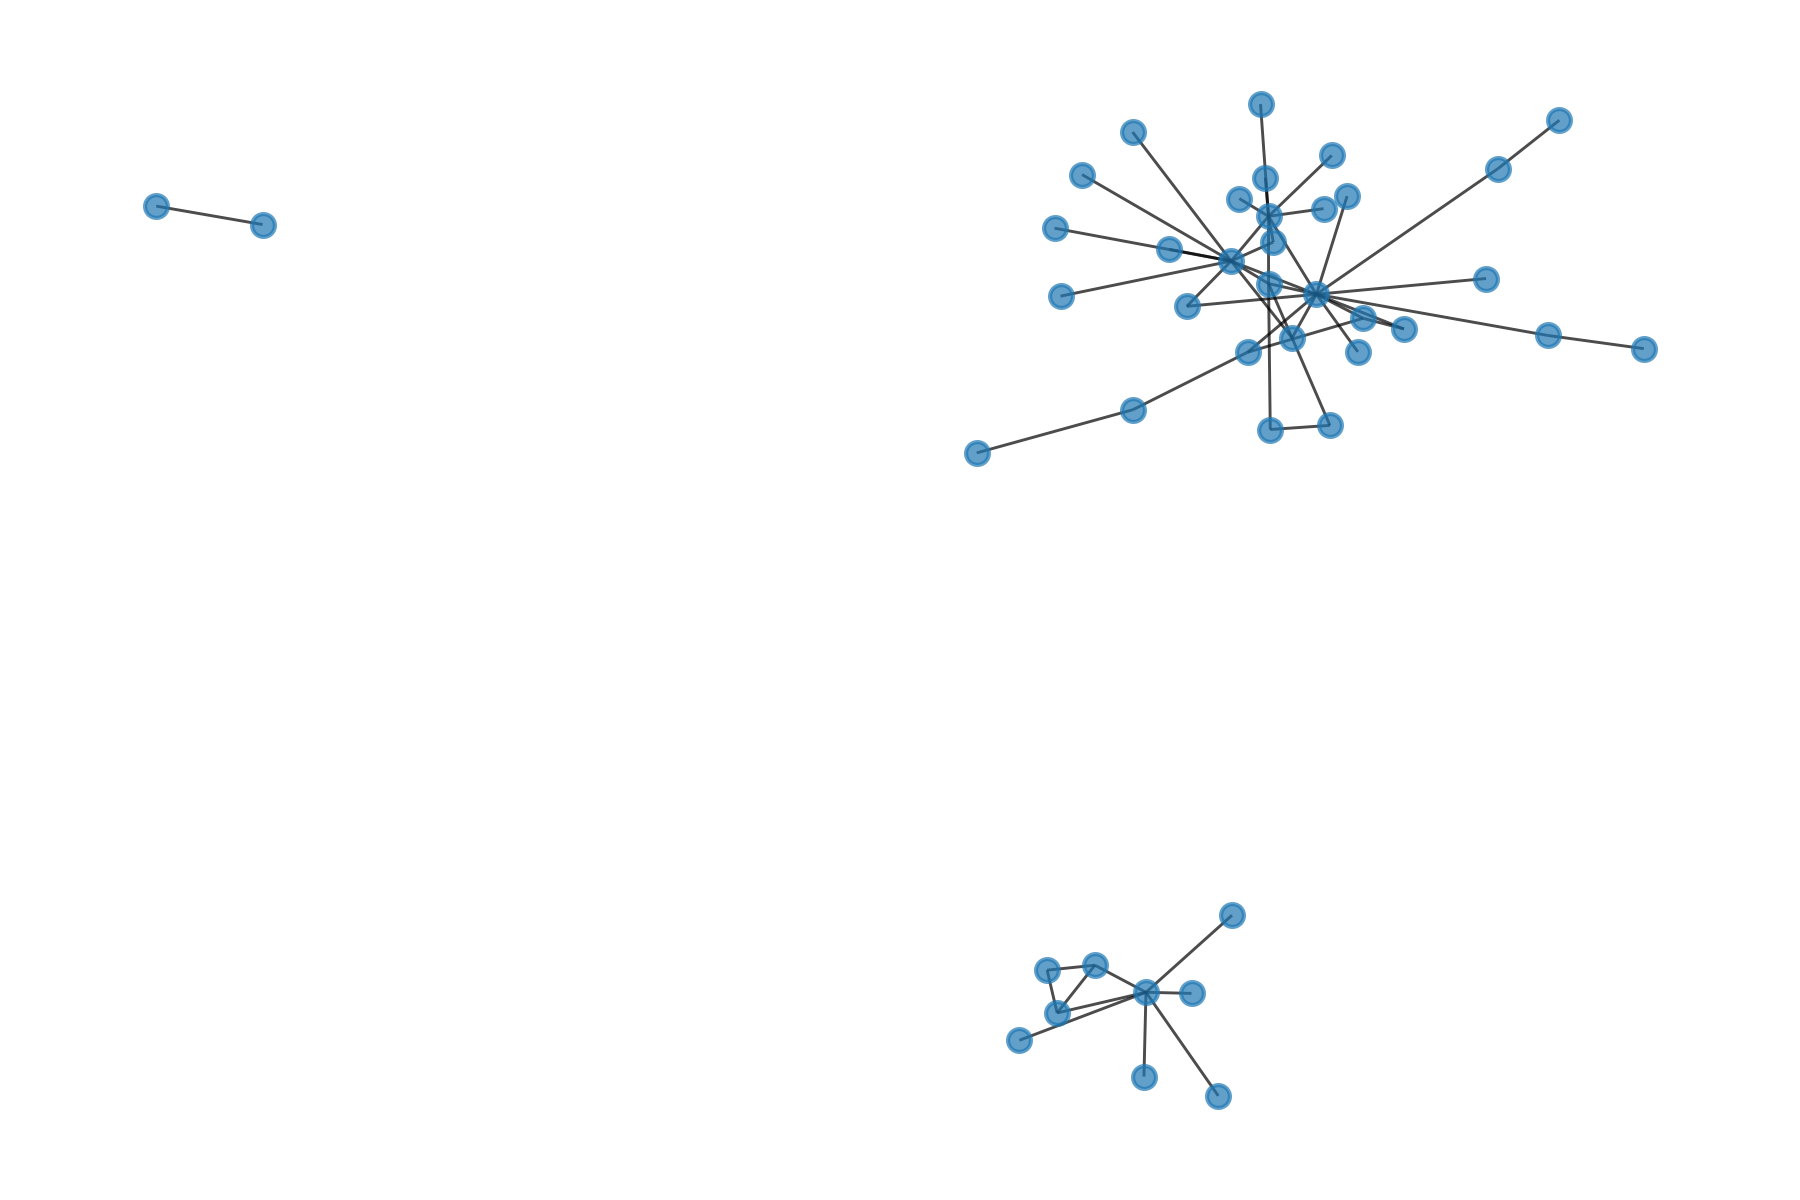
\includegraphics[width=1\linewidth]{problem_02/network_phase10}
	\end{minipage}
	\begin{minipage}{.24\textwidth}
		\centering
		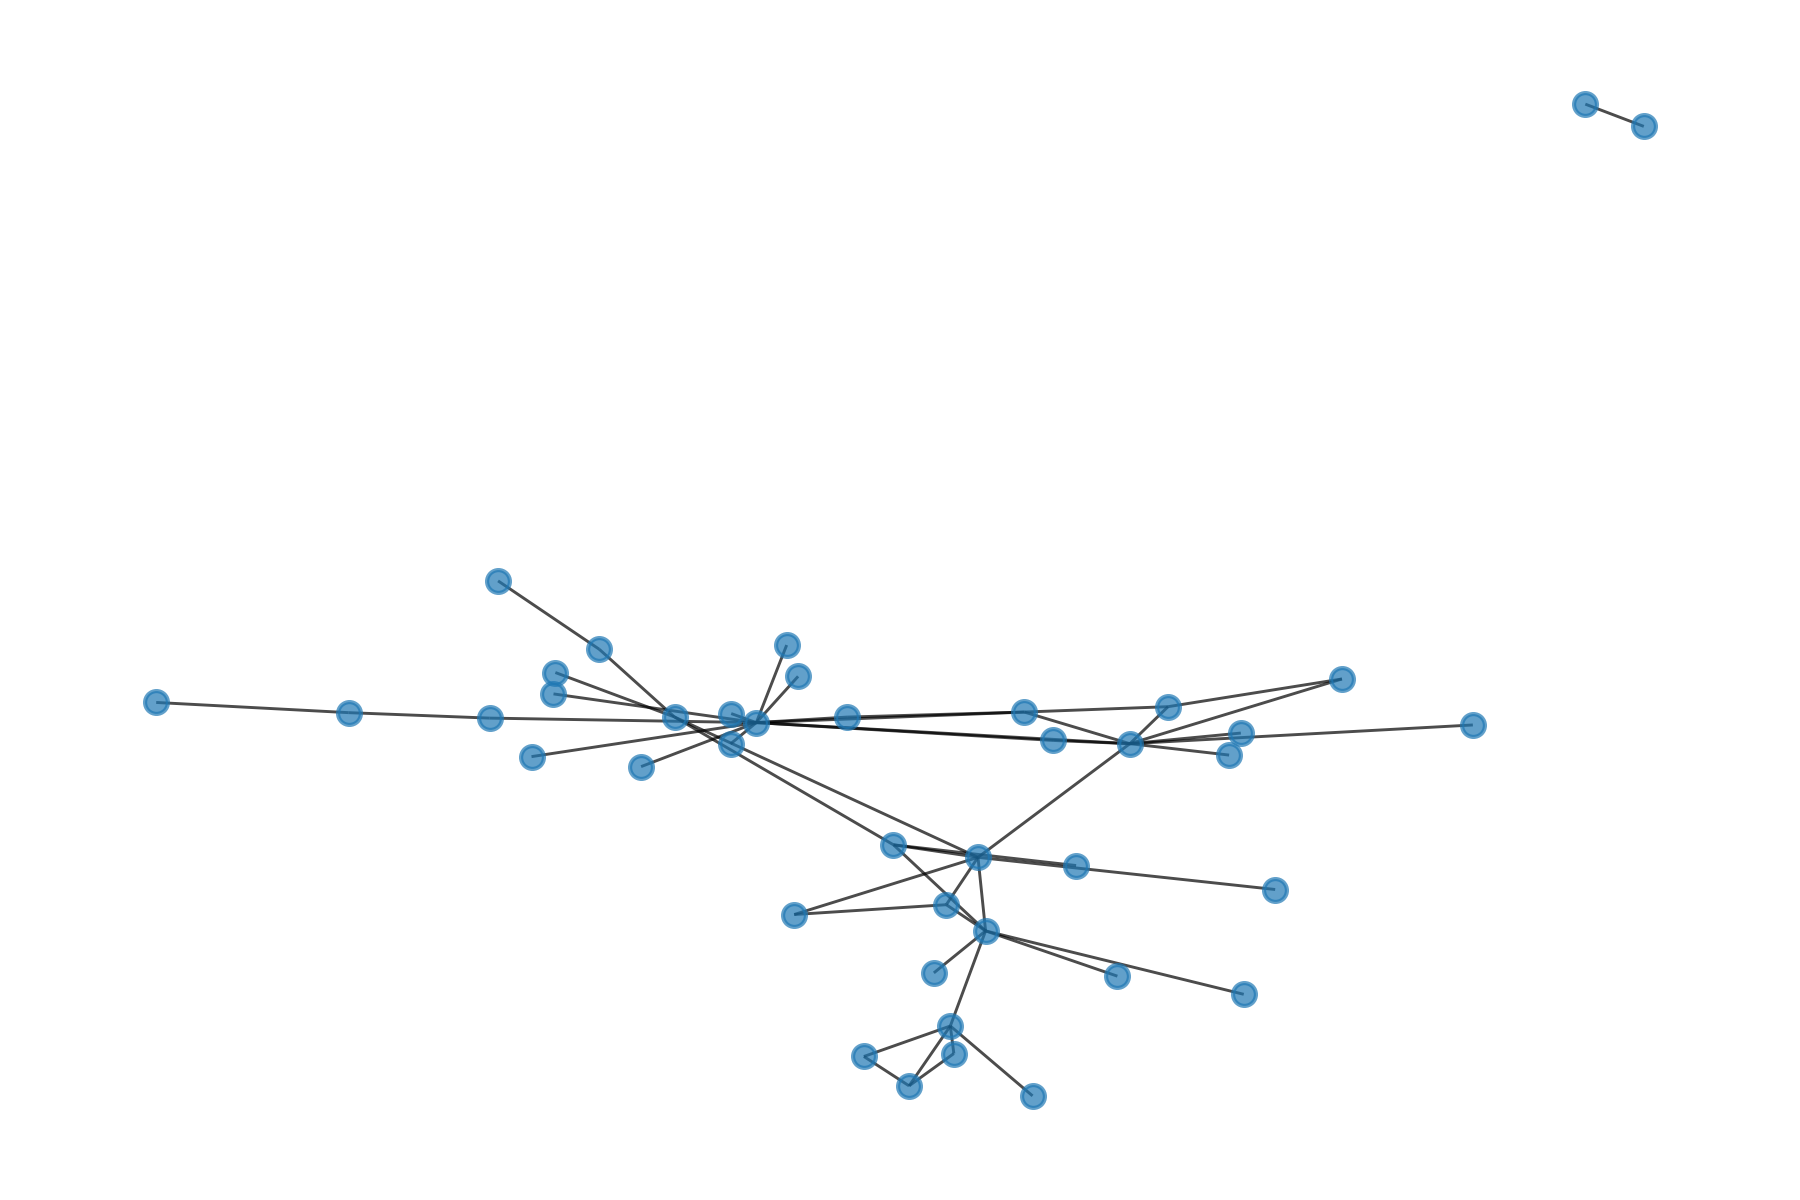
\includegraphics[width=1\linewidth]{problem_02/network_phase11}
	\end{minipage}
	\caption{CAVIAR network visualization over different phases (from left to right, from top to bottom: phase 1,..., phase 11, without node labels)}
	\label{fig:network_visualization}
\end{figure}

\begin{figure}[htbp]
	\centering
	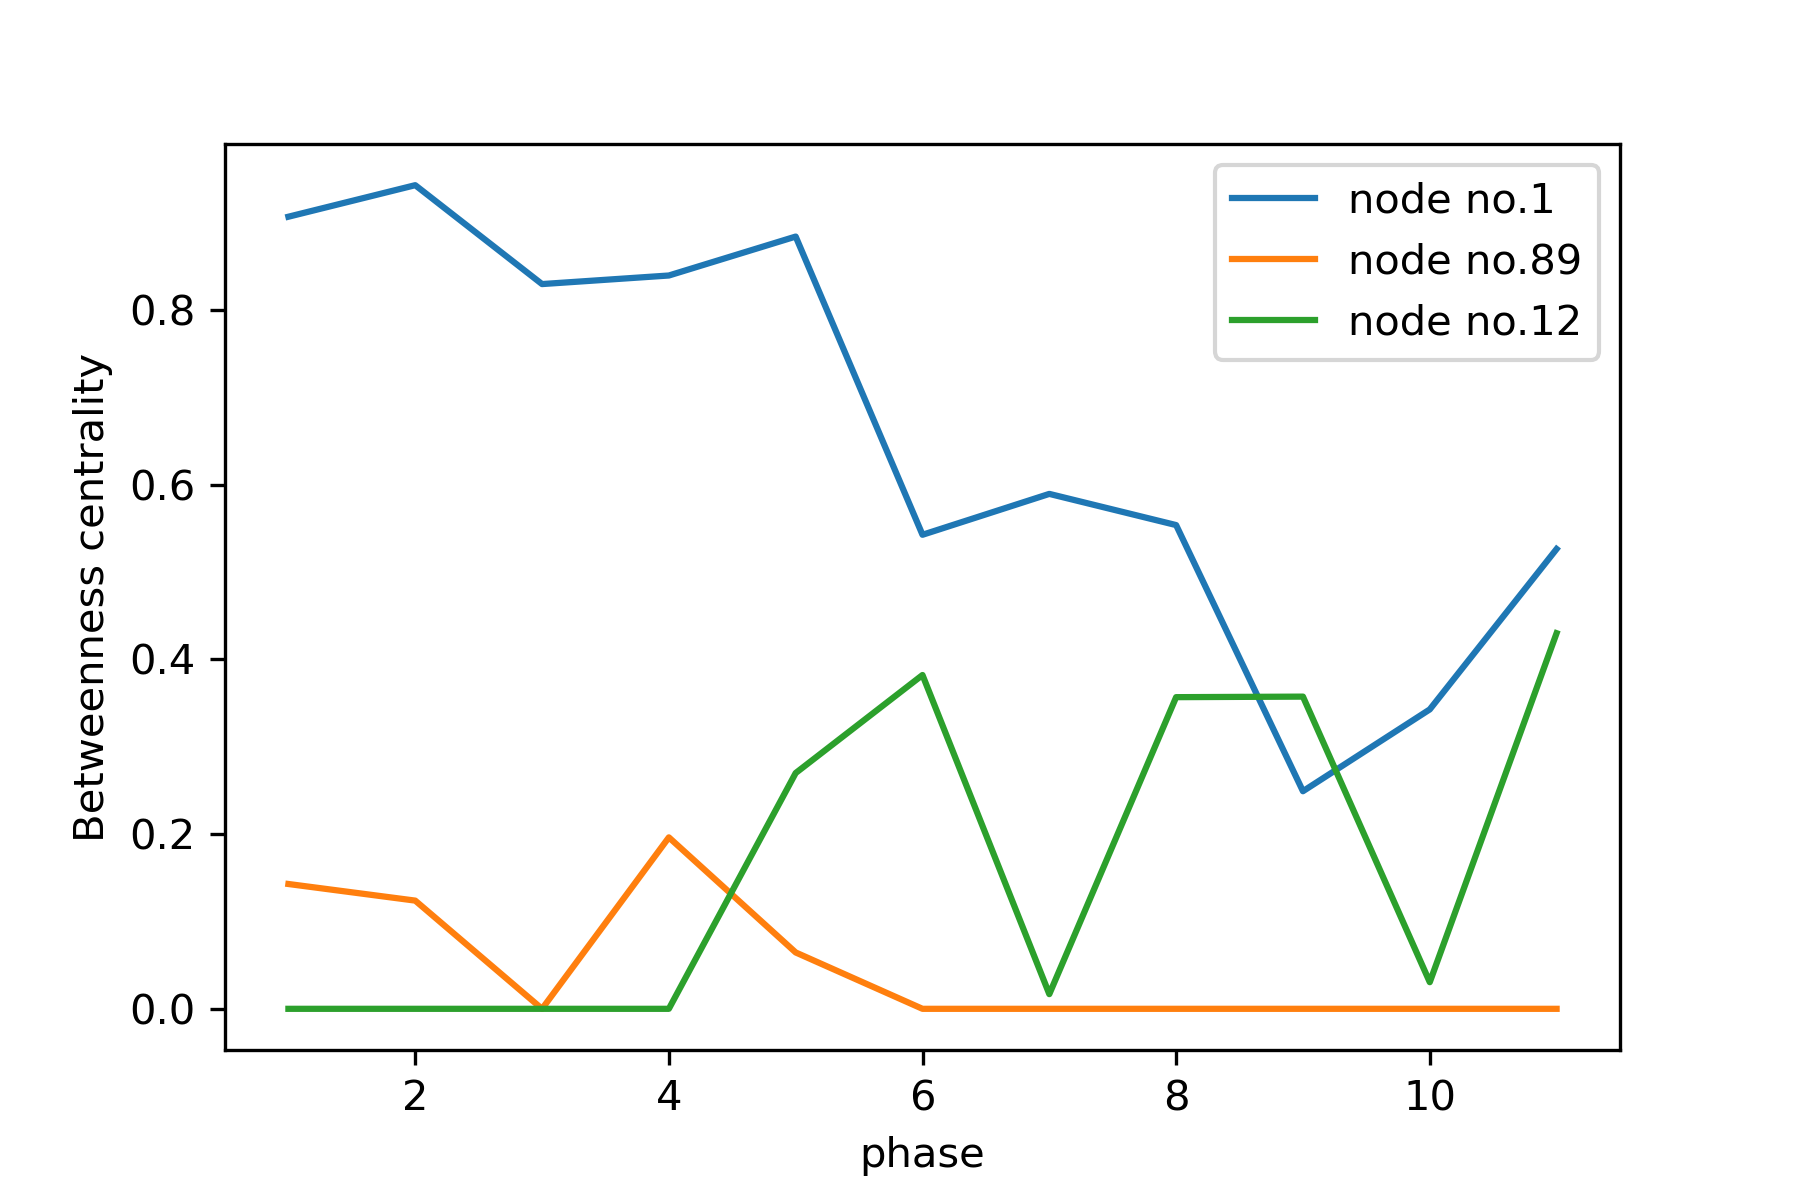
\includegraphics[width=0.7\linewidth]{problem_02/betweenness_specific_nodes}
	\caption{Betweenness centrality of specific nodes over phases}
	\label{fig:betweenness_specific_nodes}
\end{figure}

There are some interesting shifts in the development to see at phases 3-4-5 and phases 8-9-10. In the first period the network responds to a seizure of 300kg marijuana in value of 2.5x$10^6$\$ in phase 4 (see figure \ref{fig:visualization_phases_3_5_labels}). Here, the node no. 89 reaches its maximum importance according to betweenness centrality as node no. 1 stays on a high level between 0.8-0.9 (see figure \ref{fig:betweenness_specific_nodes}).\\

\begin{figure}[htbp]
	\centering
	\begin{minipage}{.32\textwidth}
		\centering
		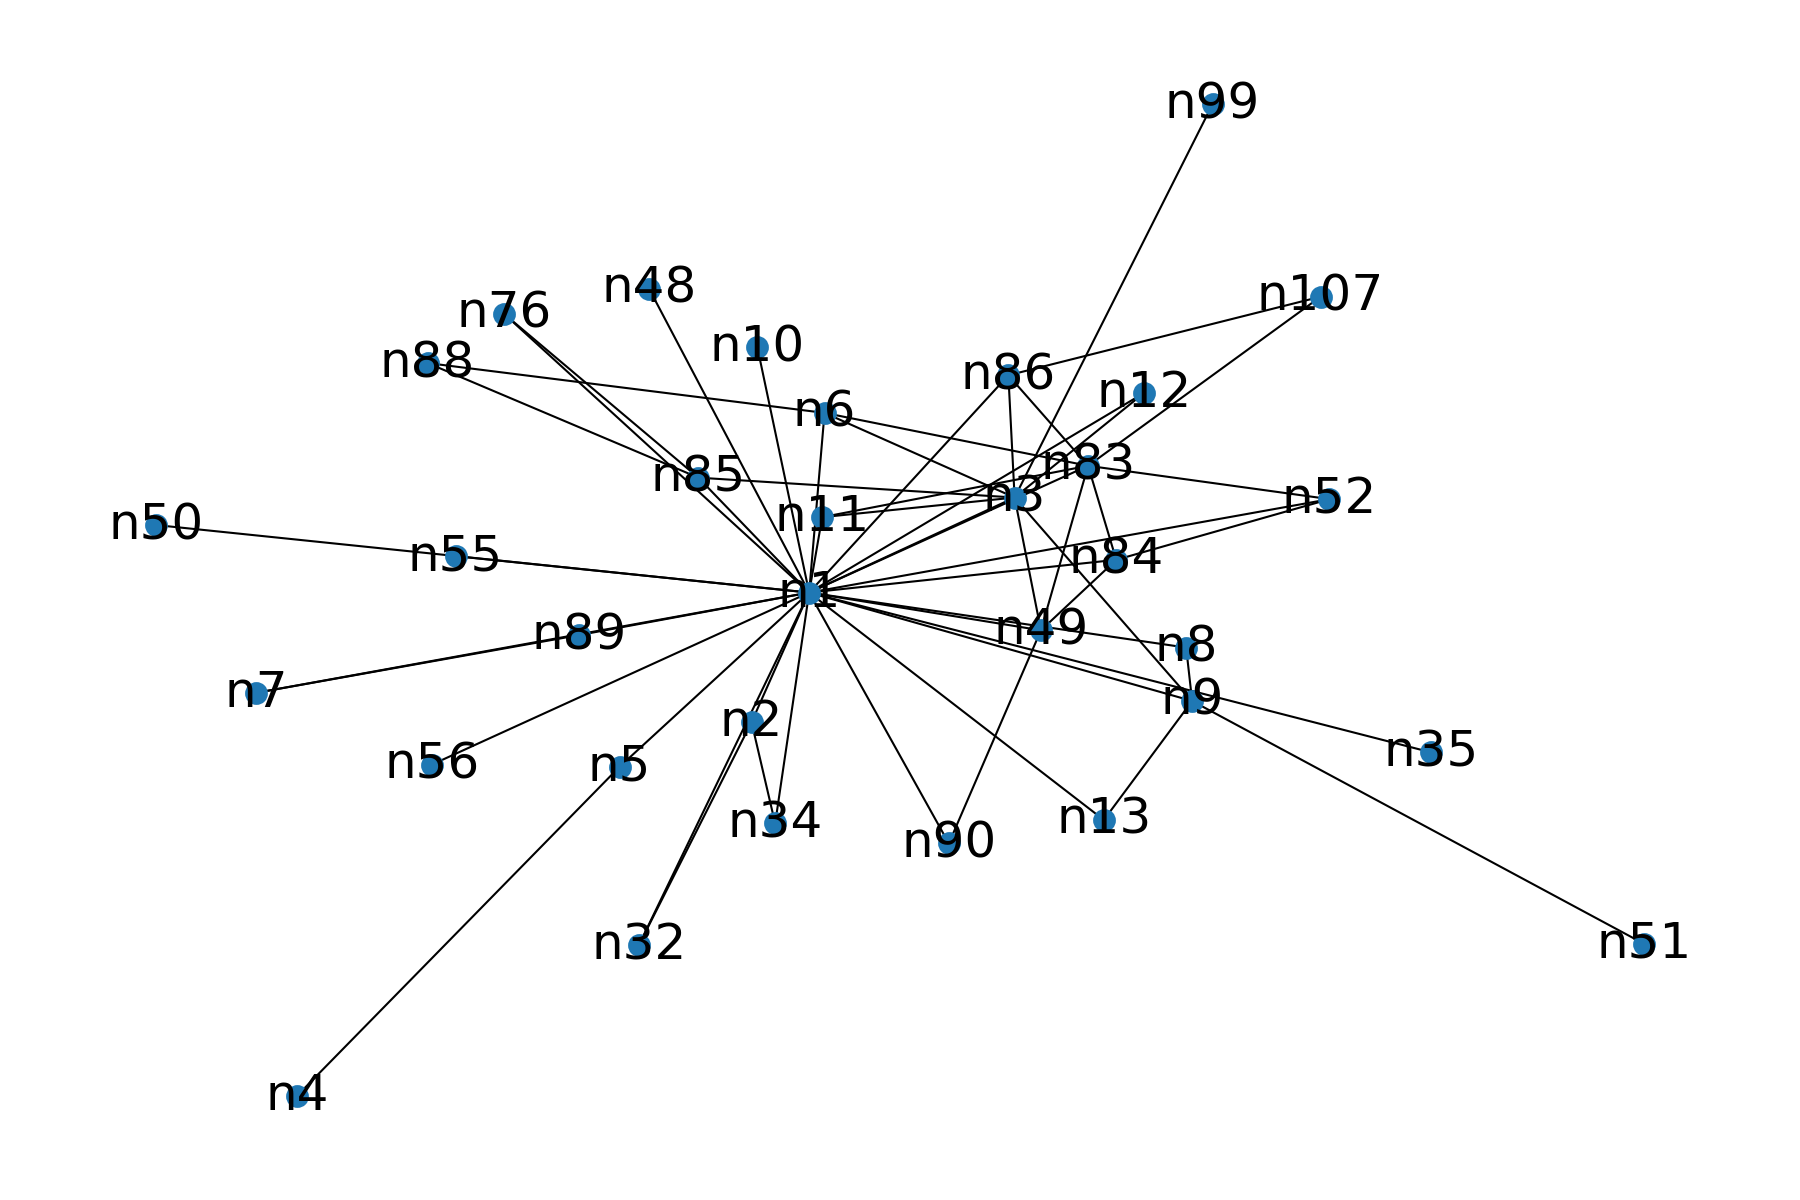
\includegraphics[width=1\linewidth]{problem_02/network_labels_phase3}
	\end{minipage}
	\begin{minipage}{.32\textwidth}
		\centering
		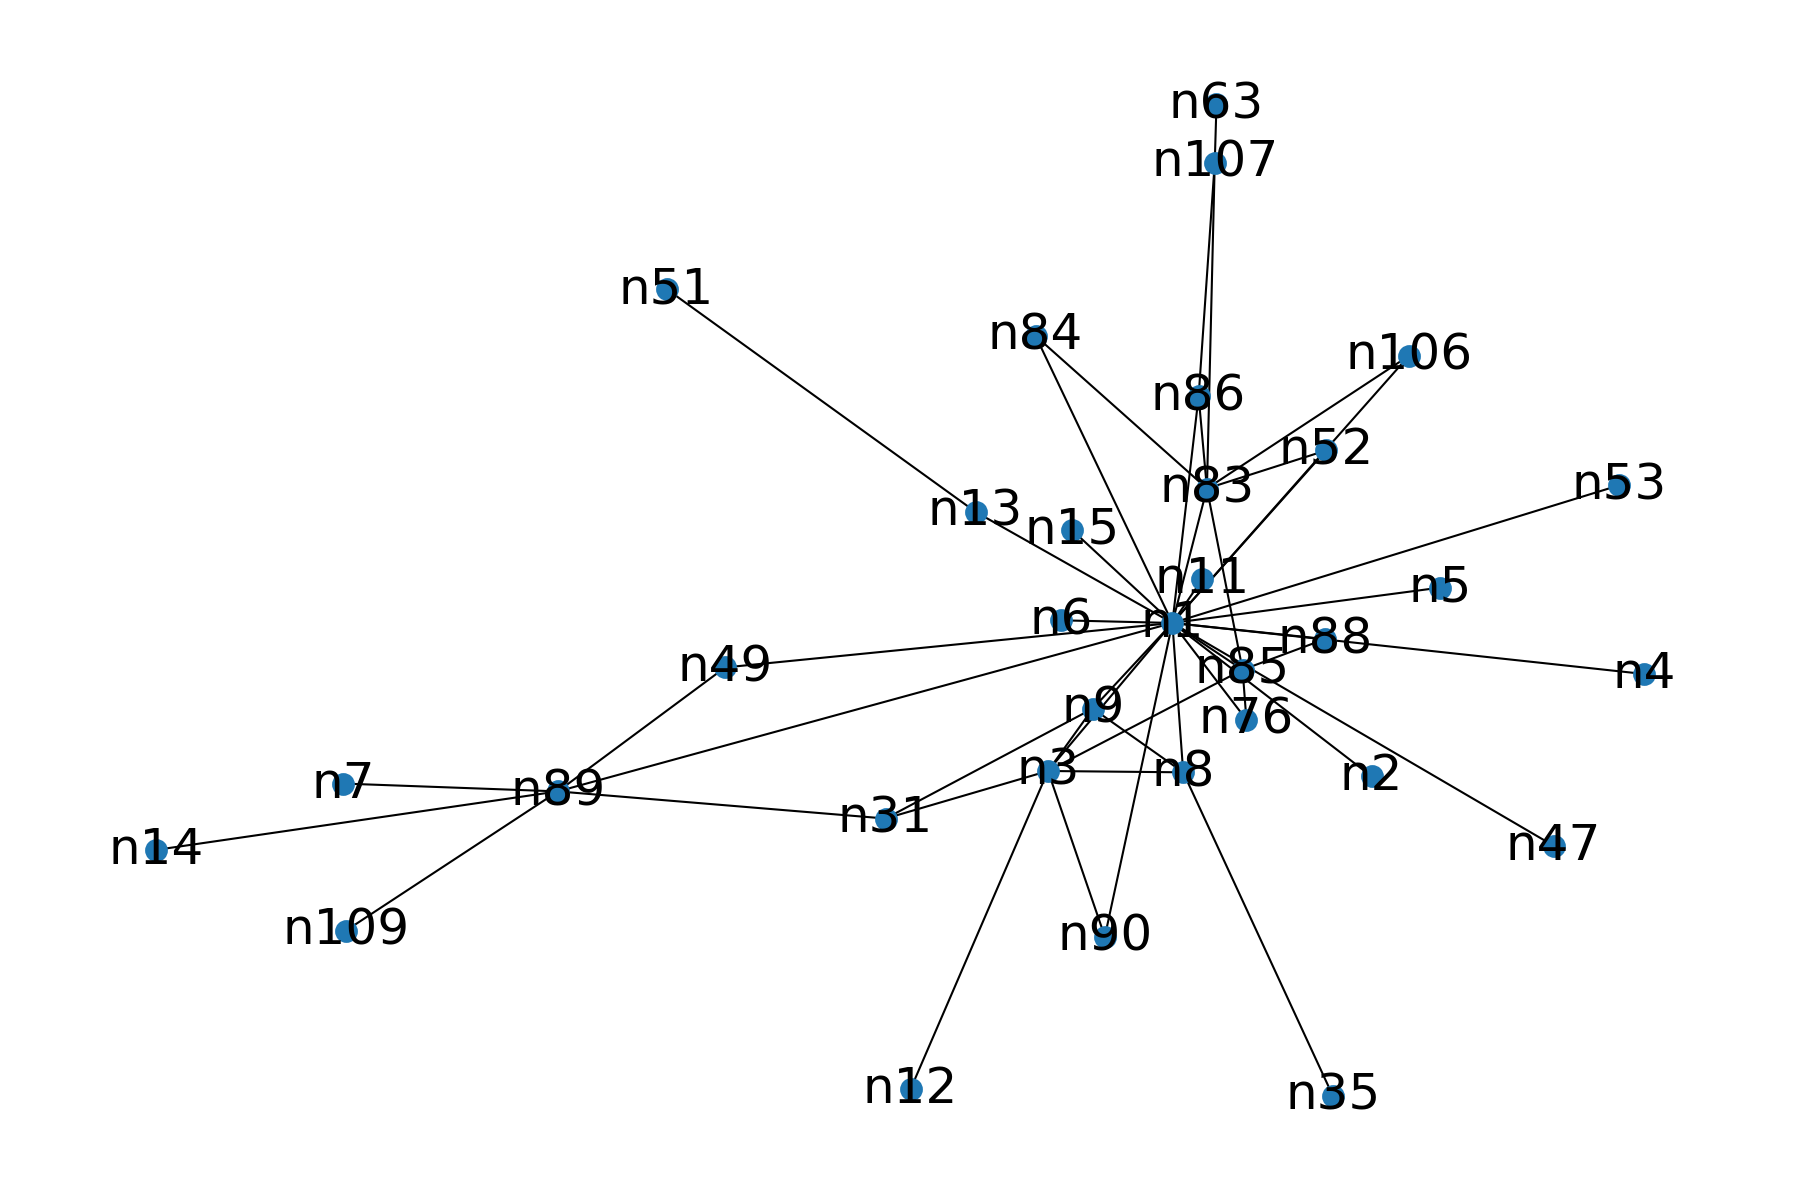
\includegraphics[width=1\linewidth]{problem_02/network_labels_phase4}
	\end{minipage}
	\begin{minipage}{.32\textwidth}
		\centering
		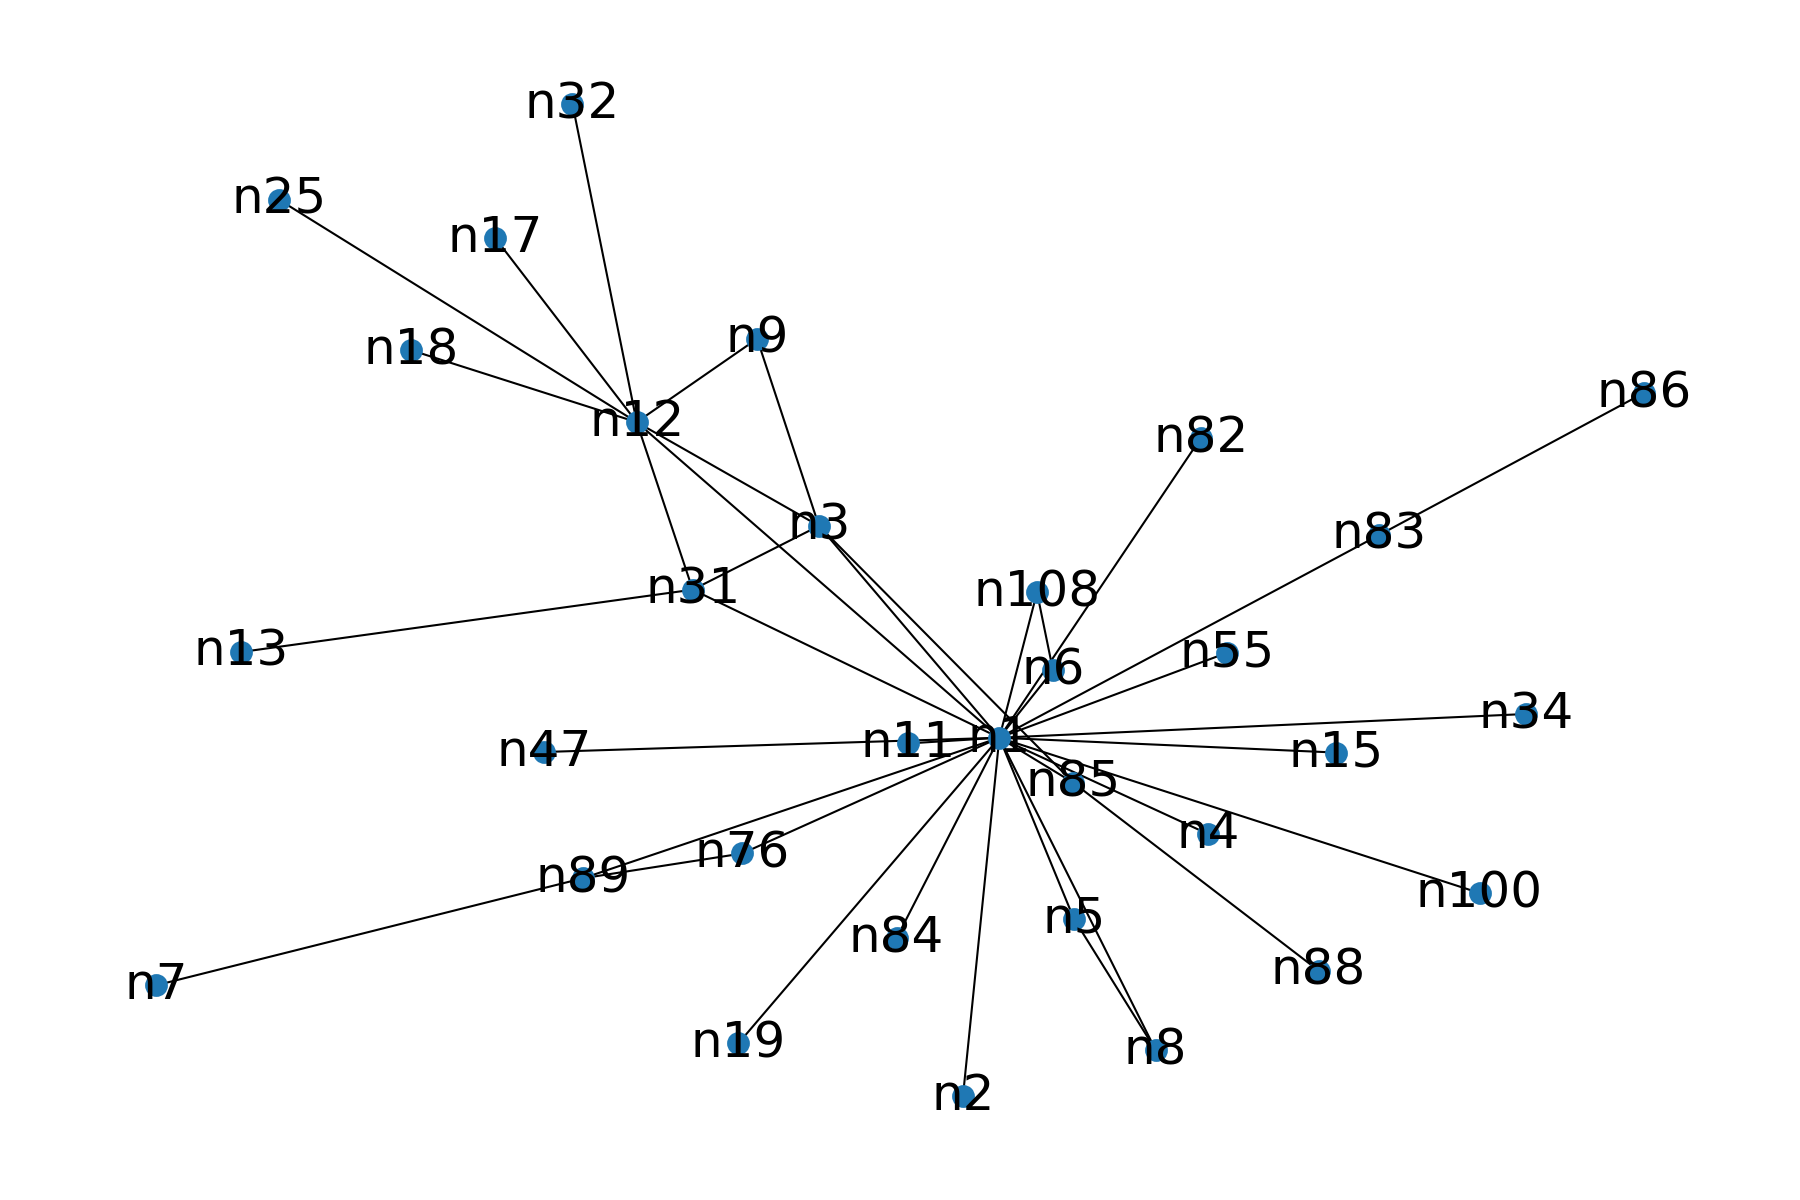
\includegraphics[width=1\linewidth]{problem_02/network_labels_phase5}
	\end{minipage}
	\caption{CAVIAR network visualization over different phases (from left to right: phase 3, phase 4, phase 5, with node labels)}
\label{fig:visualization_phases_3_5_labels}
\end{figure}

The second period around the phases 8, 9 and 10 is significant as well (see figure \ref{fig:visualization_phases_8_10_labels}). Here, multiple seizures were done: Cocaine in value of 360x$10^3$\$ (phase 8) and cocaine and marijuana in total value of 4.3x$10^6$\$ (phase 9). This is the period in which node no. 1 reaches its minimum importance according to betweenness centrality whereas node no. 12 reaches its maximum (see figure \ref{fig:betweenness_specific_nodes}). In phase 10 node no. 12 is a central node for one separated small network.\\

\begin{figure}[htbp]
	\centering
	\begin{minipage}{.32\textwidth}
		\centering
		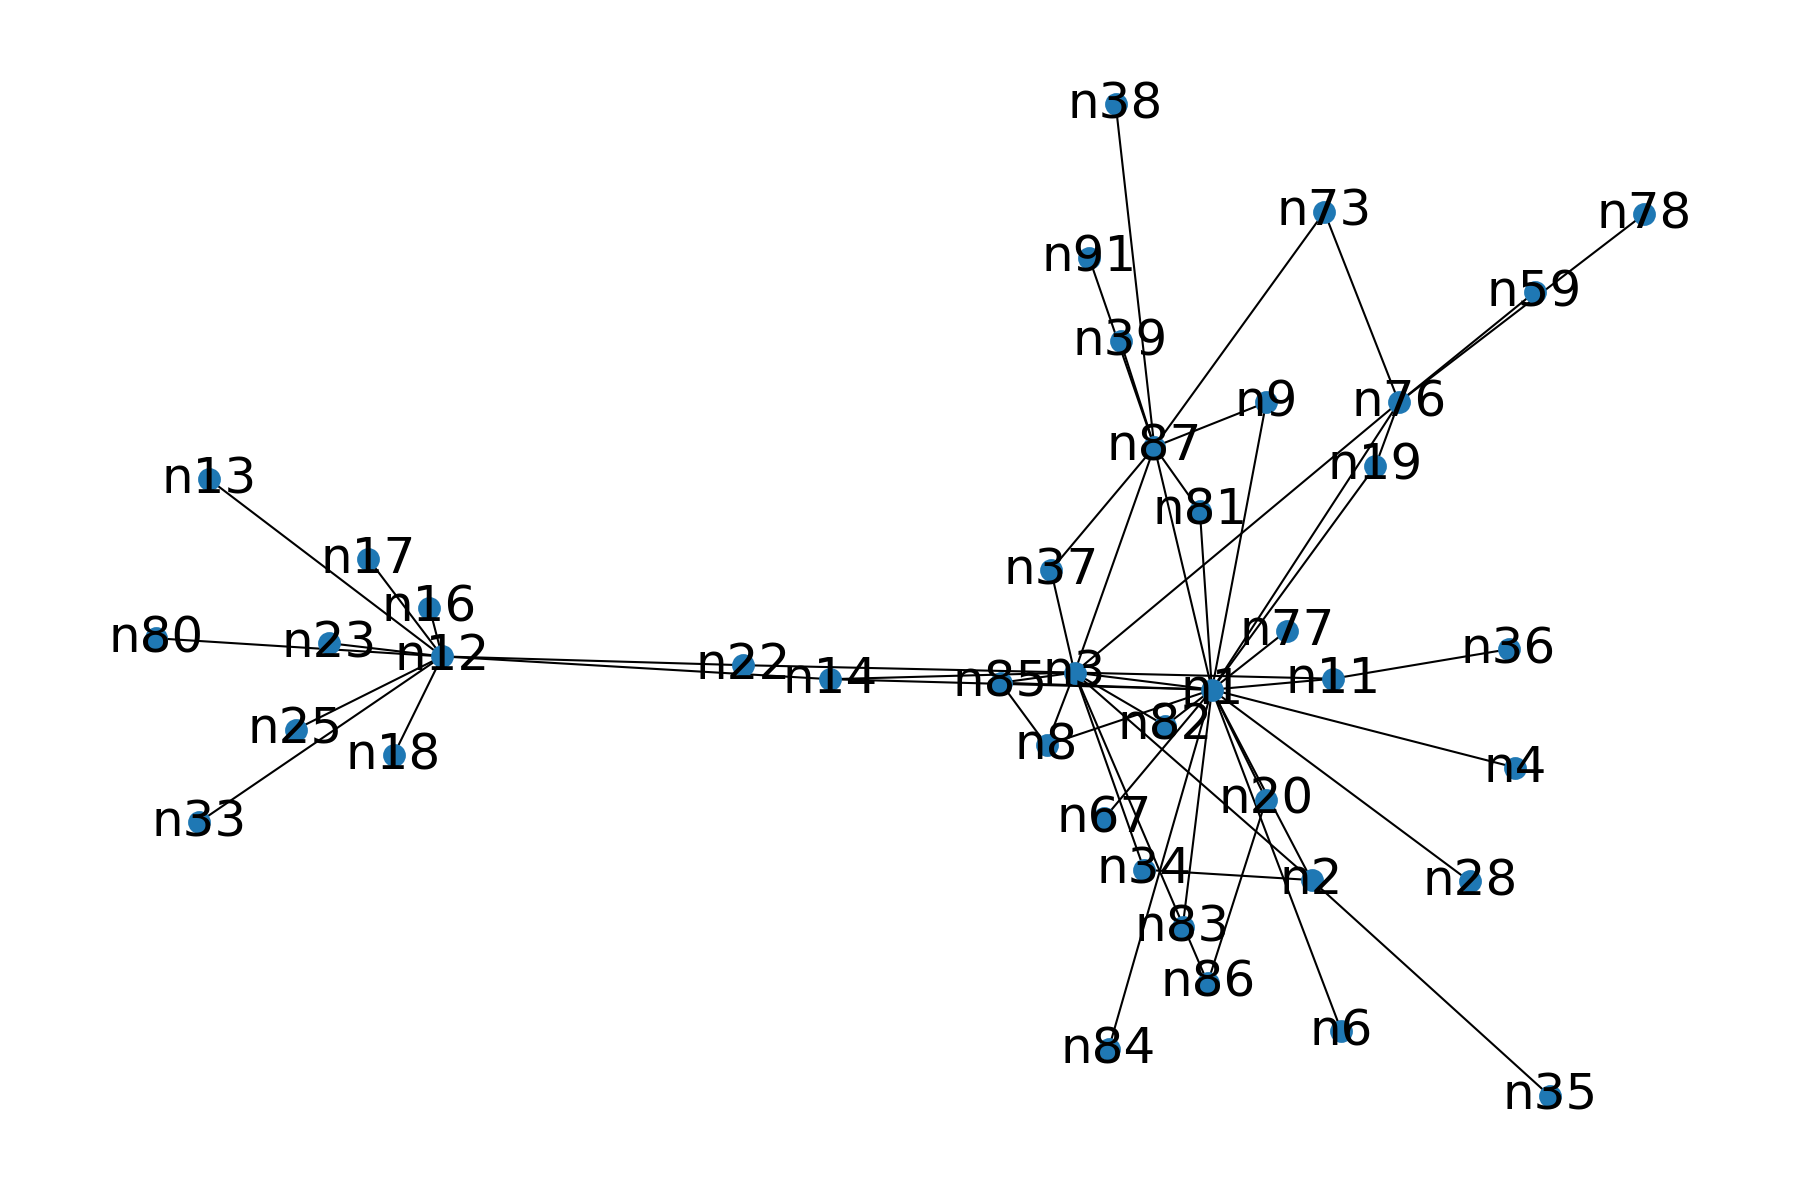
\includegraphics[width=1\linewidth]{problem_02/network_labels_phase8}
	\end{minipage}
	\begin{minipage}{.32\textwidth}
		\centering
		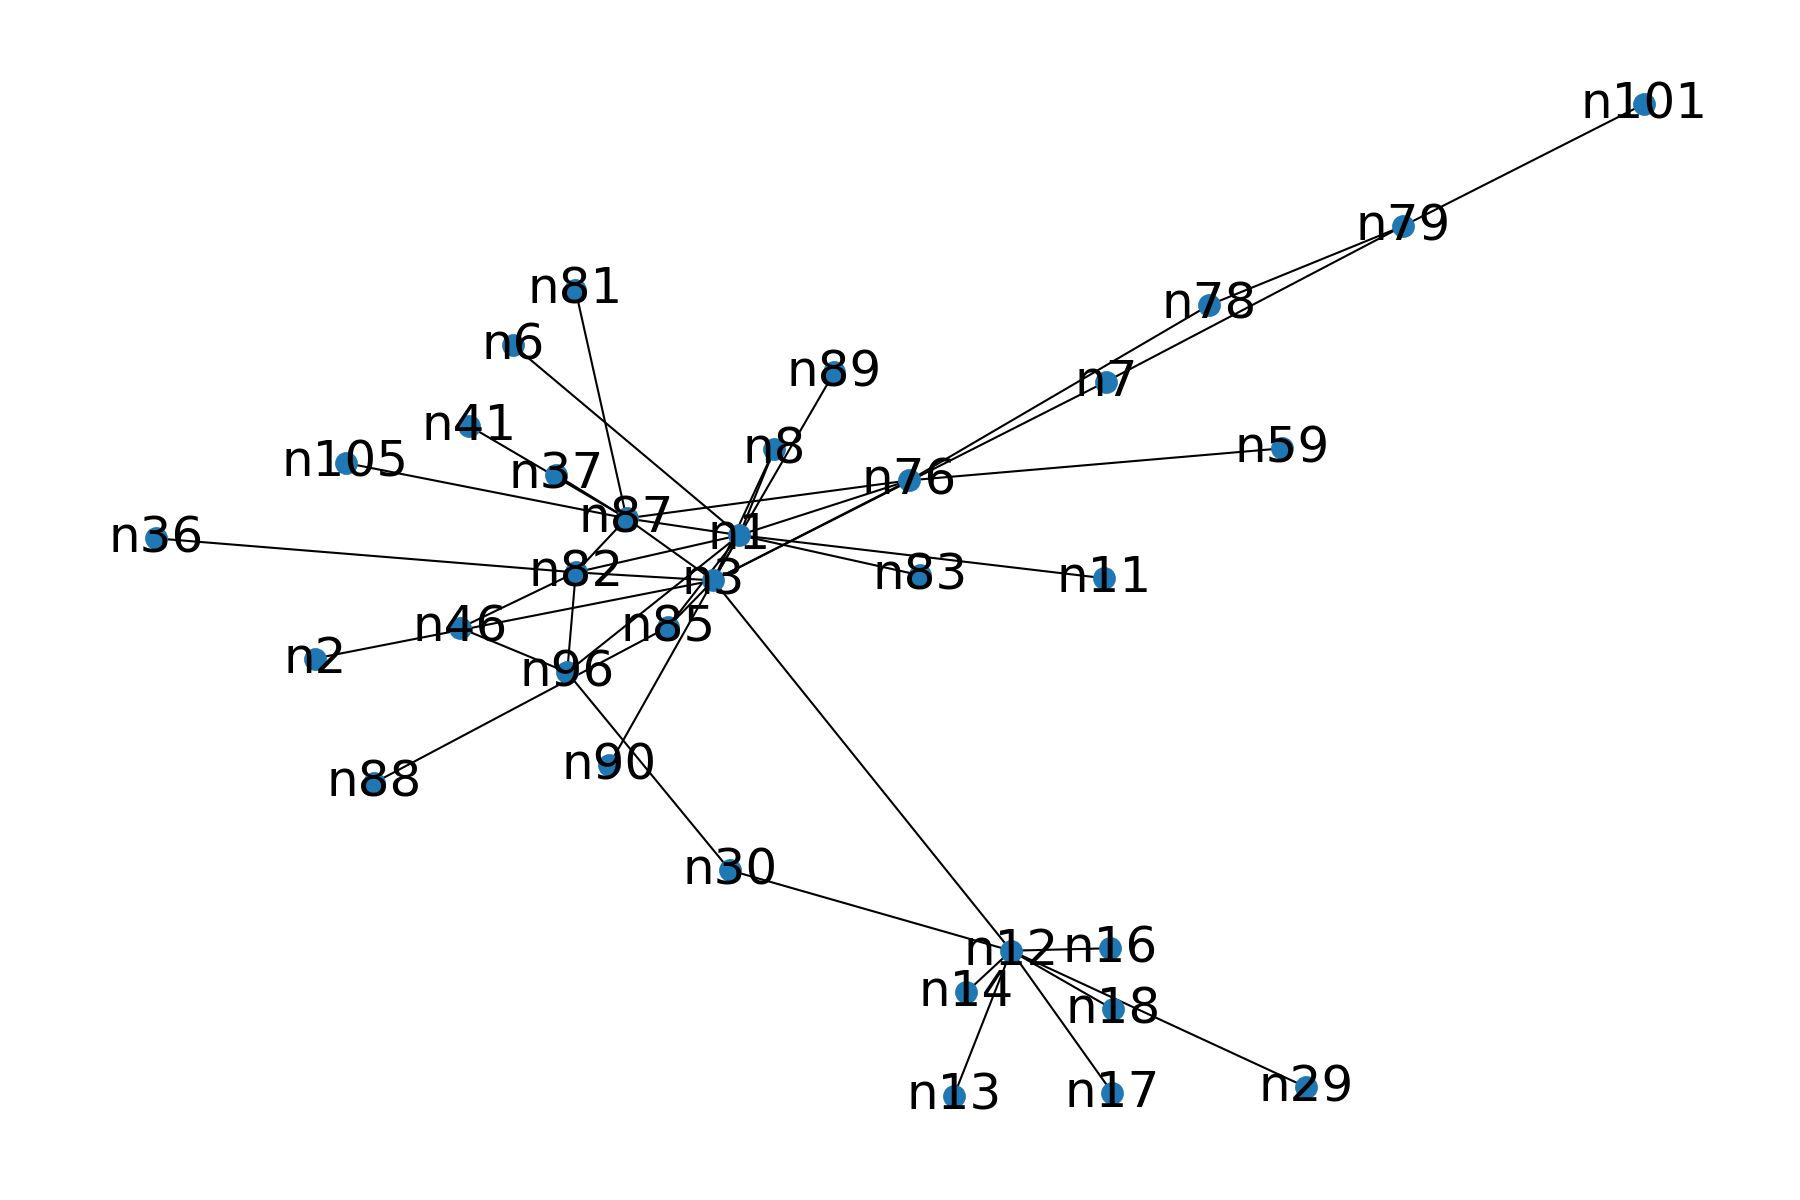
\includegraphics[width=1\linewidth]{problem_02/network_labels_phase9}
	\end{minipage}
	\begin{minipage}{.32\textwidth}
		\centering
		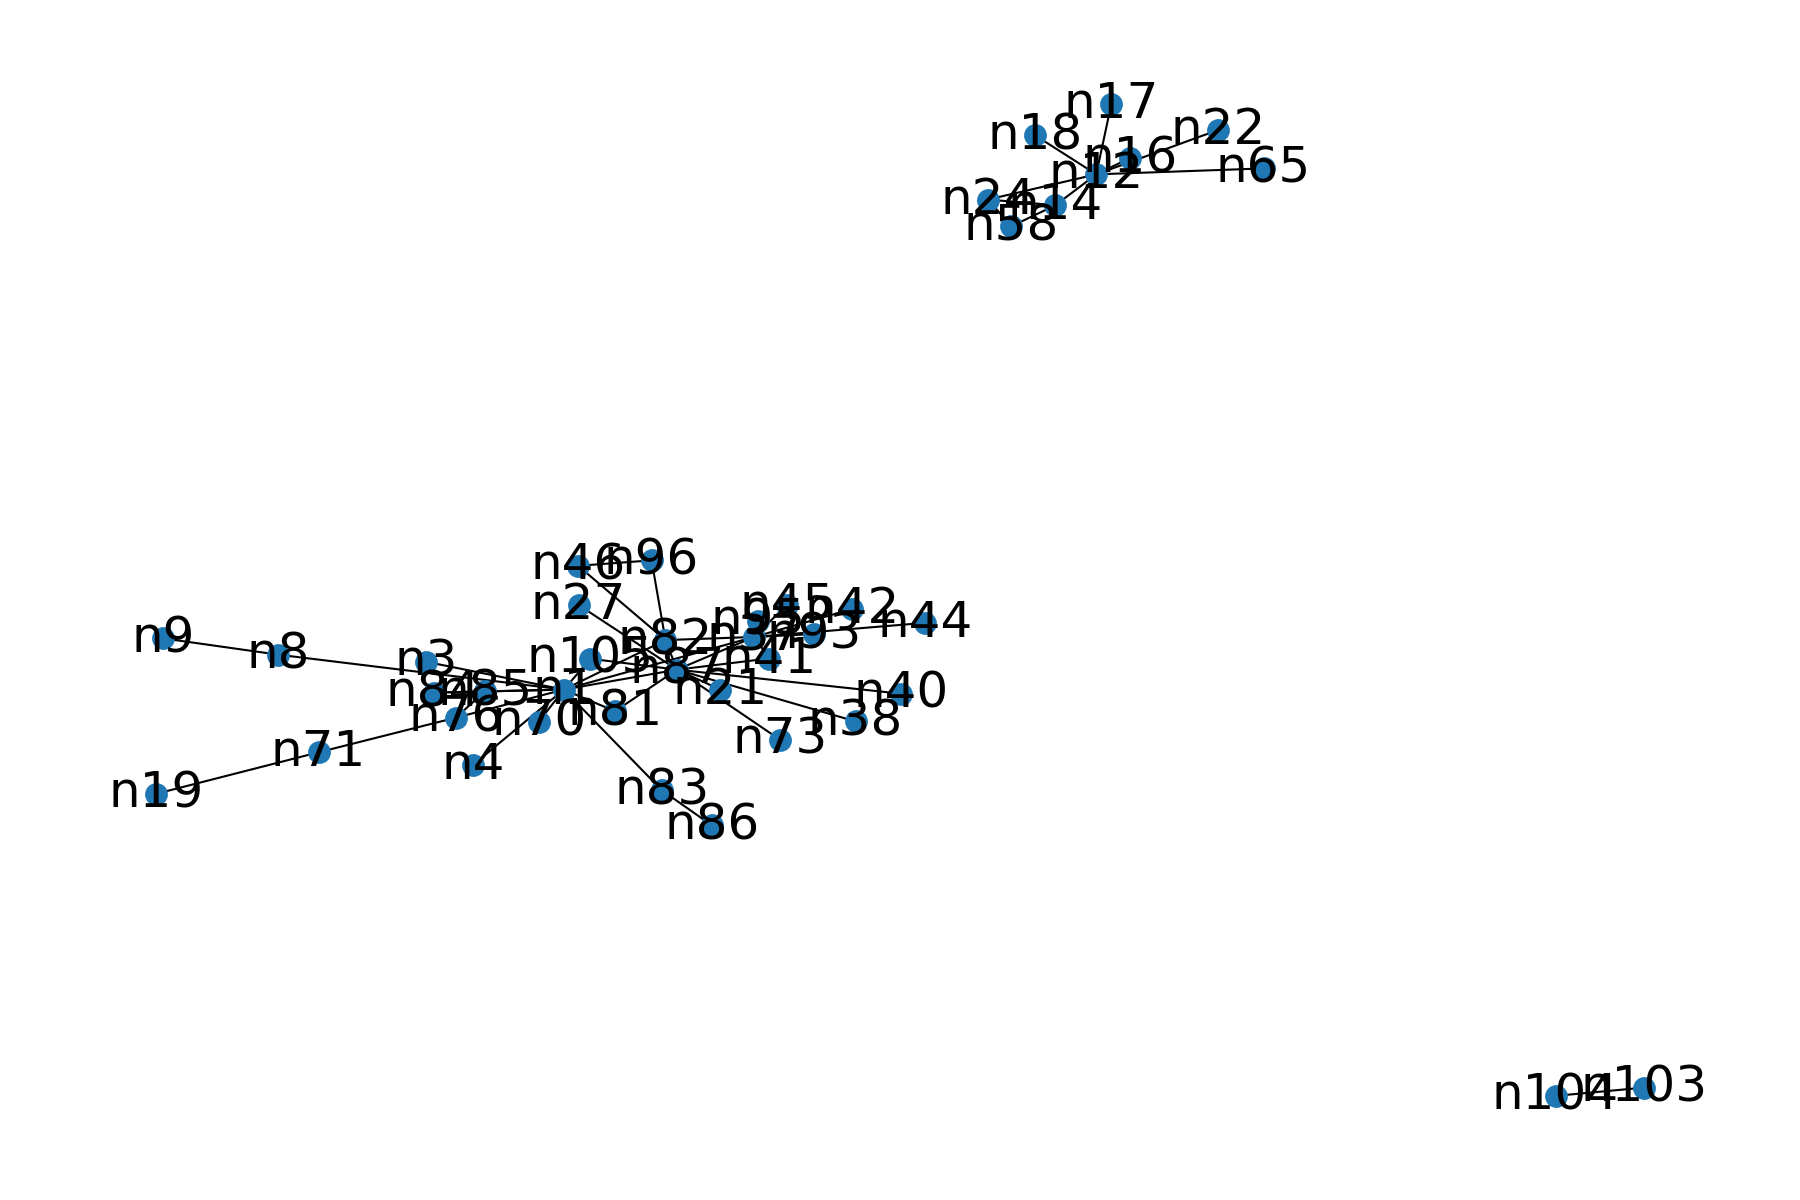
\includegraphics[width=1\linewidth]{problem_02/network_labels_phase10}
	\end{minipage}
	\caption{CAVIAR network visualization over different phases (from left to right: phase 8, phase 9, phase 10, with node labels)}
	\label{fig:visualization_phases_8_10_labels}
\end{figure}